% !Mode:: "TeX:UTF-8"
\chapter{Методы генерации ограничений для описания поведения тестовых программ}

\section{Модель модулей управления памятью --- ???}

Для построения ограничений необходимо описать семантику инструкций и модель состояния микропроцессора. Описание семантики инструкции предлагается проводить в виде текста на специальном императивном языке. Этот язык по большей части основан на том описании, как оно дается в документации по архитектуре микропрцоессора (т.е. его системе инструкций), например, в~\cite{mips64_II}.

%Данная работа по разработке методов построения программ по тестовым
%шаблонам выполнялась в рамках \emph{подхода, основанного на
%моделях}. А именно для автоматического построения тестовой программы
%строится набор моделей, описывающих особенности архитектуры
%микропроцессора, и запускается генератор, который на основе шаблона
%и моделей строит программы. В данной работе используются следующие
%модели:
%\begin{itemize}
%  \item \emph{модель инструкции} описывает операционную семантику
%  инструкции (точнее, ветви функциональности инструкции);
%  \item \emph{модель модуля управления памятью} описывает механизмы
%  и ситуации в работе модуля управления памятью.
%\end{itemize}
%
%На рисунке~\ref{scheme_program_building} показана общая схема
%построения тестовой программы с использованием моделей, предлагаемая
%в данной работе:
%\begin{enumerate}
%    \item для каждой инструкции тестового шаблона составляется
%    модель инструкции (на рисунке~\ref{scheme_program_building}
%    такой инструкцией является \texttt{LOAD});
%    \item составляется модель модуля управления памятью, в которую
%    входит \emph{структурная модель} модуля управления памятью и
%    \emph{генератор ограничений};
%    \item на основе подготовленных моделей моделе-независимый
%    генератор строит систему ограничений и вызывает внешний решатель
%    ограничений для этой системы;
%    \item на основе <<модели ограничений>>, построенной решателем,
%    (моделью ограничений является отображение имен переменных
%    ограничений в значения) строится тестовая программа, а именно,
%    генерируются инициализирующие инструкции и инструкции тестового воздействия, возможно с
%    подстановкой значений на место некоторых параметров.
%\end{enumerate}
%
%\begin{figure}[h] \center
%  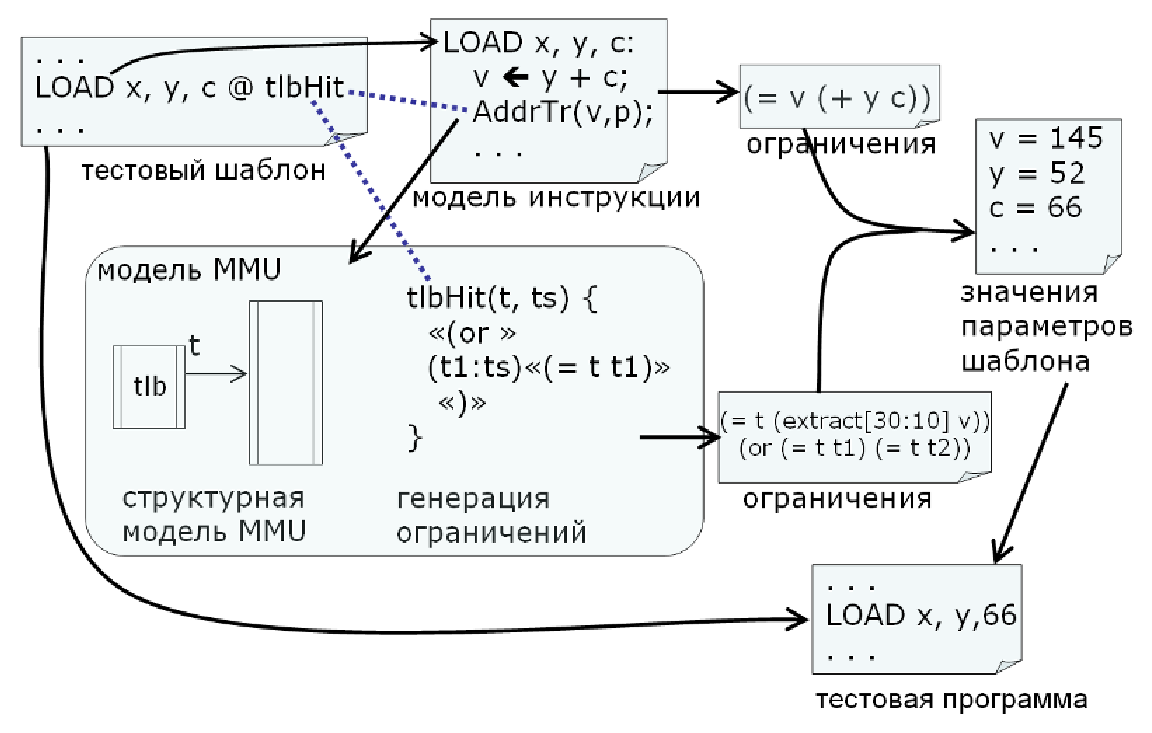
\includegraphics[width=0.9\textwidth]{2.theor/wholesheme}\\
%  \caption{Общая схема построения тестовой
%  программы}\label{scheme_program_building}
%\end{figure}
%
%\subsection{Модели инструкций}

пример + его пояснение

связь с меткой в тестовом шаблоне (+ что это ветви документации)

\emph{Модель инструкции} описывает ветвь функциональности в виде
последовательности операторов (присваивание, допущение (assume),
вызов процедуры), ветвление внутри модели инструкции в явном виде
отсутствует. На рисунке~\ref{inst_model_example} дан пример модели
инструкции \texttt{LOADWORD x, y, c} в микропроцессорах архитектуры
\textsc{MIPS64} (эта инструкция загружает в регистр \texttt{x} 32
байта основной памяти по адресу, содержащемуся в регистре \texttt{y}
с учетом смещения \texttt{c}). Первый оператор (оператор
присваивания) присваивает новой переменной \texttt{vAddr} значение
виртуального адреса в инструкции. Следующий оператор (2) (допущение)
проверяет выравнивание виртуального адреса: для загрузки 32 байт
адрес должен быть кратен 4. Следующий оператор (3) -- вызов
процедуры \texttt{AddressTranslation}, он помещает в переменную
\texttt{pAddr} физический адрес, соответствующий виртуальному адресу
\texttt{vAddr}, причем трансляция адреса должна пройти до конца. И
так далее. \emph{Процедурой} будем называть неделимое обращение к
модулю управления памяти (например, трансляция адреса, обращение в
основную память через кэш-память).

\begin{figure}[h]\center
\begin{verbatim}
  (1) vAddr <- y + (64)c;
  (2) assume vAddr[1:0] == 0;
  (3) AddressTranslation(vAddr, pAddr, DATA, LOAD);
  (4) pAddr <- pAddr[35:3] || (pAddr[2] + 1) || pAddr[1:0];
  (5) LoadMemory(memdw, pAddr, vAddr, DATA, WORD);
  (6) x <- 0^32 || memdw[vAddr[2:0]];
\end{verbatim}
\caption{Модель инструкции <<LOADWORD x, y, c>> в микропроцессоре
архитектуры MIPS64}\label{inst_model_example}
\end{figure}

Модели инструкций извлекаются из документации по архитектуре
(например,~\cite{mips64_II}) и по результатам общения с
разработчиками микропроцессора.

Модели инструкций используются для указания зависимостей значений
аргументов инструкции. Эти зависимости выражаются в виде ограничений
(constraints) и используются решатели ограничений для получения
значений аргументов инструкций. На основе полученных значений будет
сформирована тестовая программа.

В диссертации генерация ограничений по моделям инструкций
осуществляется с помощью известный метода, т.н. символьного
исполнения моделей инструкций~\cite{my_syrcose_2008}. Каждой
переменной модели инструкций ставится в соответствие набор
переменных, не меняющих своё значение. Такие новые переменные
позволяют однозначно восстановить значения переменных модели
инструкций (т.е. и значения аргументов инструкции). Ограничения
формулируются на введенных переменных: каждый оператор модели
инструкции транслируется в некоторый набор ограничений.

Операторы присваивания и допущения выражаются на языке, независимом
от модулей управления памятью. Для этих операторов трансляция в
ограничения производится полностью автоматически. Трансляция вызовов
процедур в ограничения зависит от механизмов работы модулей
управления памятью. Эта трансляция и составляет основу \emph{модели
модуля управления памятью}.

Введение собственной модели для модуля управления памятью
преследовало несколько целей. Во-первых, это ввести терминологию для
дальнейшего описания методов генерации ограничений для тестовых
шаблонов. И, во-вторых, выделить класс архитектур микропроцессоров,
для которых предлагаемые далее методы генерации ограничений
применимы (а именно, методы применимы тогда, когда можно построить
модель).

Модель модуля управления памятью отражает только те особенности
модуля управления памятью, на которые нацелено проводимое
тестирование. Например, если микропроцессор включает иерархические
таблицы страниц, но в тестовом шаблоне нет тестовых ситуаций таблицы
отдельных уровней (а содержит тестовые ситуации на все таблицы
целиком), то в модели такая таблица будет представлена без иерархии,
целиком. Кроме того, в микропроцессоре могут быть реализованы
механизмы, меняющие порядок исполнения инструкций по сравнению с
программой (спекулятивное выполнение, предсказание
переходов~\cite{Pasko}), однако их учитывать в данном тестировании
не имеет смысла, ибо в таком случае невозможно будет провести
тестирование (если неизвестен порядок инструкций, то невозможно
построить тестовый оракул).

\subsection{Модель состояния модулей управления памятью}

В данной работе особо важным классом инструкций в тестовых шаблонах
является класс инструкций обращения к памяти. Такие инструкции
присутствуют практически во всех микропроцессорах. Инструкции
обращения к памяти делятся на два класса: \emph{инструкции загрузки
данных из памяти} и \emph{инструкции сохранения данных в памяти}.
При исполнении такой инструкции кроме оперативной памяти могут быть
задействованы некоторые специальные структуры данных-подсистемы
микропроцессора --- а именно \emph{кэширующие буфера} и
\emph{таблицы}. Они образуют \emph{структурную модель}.

Таблицы содержат последовательный индексированный набор данных.
Изменение содержимого таблиц осуществляется только программно.
Пример таблицы -- таблица страниц виртуальной памяти. Изменение
содержимого этих таблиц может осуществляться операционной системой.

Кэширующие буфера содержат множество пар (ячеек) <<(тег, значение)>>
заданного количества. Содержимое кэширующего буфера может меняться в
процессе работы микропроцессора: какие-то ячейки добавляются,
какие-то \emph{вытесняются}. Управление кэширующими буферами
осуществляется только микропроцессором. Исполнение инструкции
обращения к памяти может включать в себя обращения к кэширующим
буферам для получения данных по некоторому тегу. Обращение к
кэширующему буферу может быть успешным (такая ситуация называется
\emph{кэш-попаданием}), если нужные данные есть в буфере, и
неуспешным (такая ситуация называется \emph{кэш-промахом}), если
нужных данных нет в буфере.

Кэширующий буфер может быть \emph{подчинен} таблице, если при
неуспешном обращении к кэширующему буферу поиск данных продолжается
в таблице, при успешном --- обращение к таблице не производится.
Если поиск в таблице оказался успешным, то найденные данные
добавляются в кэширующий буфер (некоторые данные из кэширующего
буфера при этом вытесняются для поддержания постоянного размера
буфера). Например, в микропроцессоре MIPS RM7000~\cite{mips64_III}
кэширующий буфер DTLB подчинен таблице JointTLB. Можно представить,
что кэш-память подчинена основной памяти, если рассматривать
основную память как таблицу, правда, основная память не является
подсистемой микропроцессора.

\begin{figure}[h] \center
  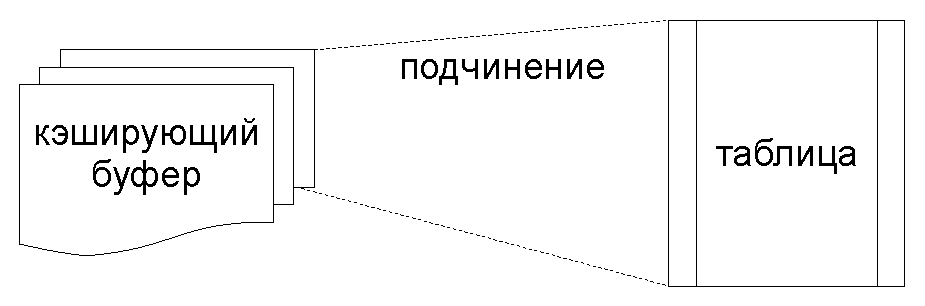
\includegraphics[width=0.6\textwidth]{2.theor/elements}\\
  \caption{Основные элементы модели модулей управления памяти}
\end{figure}

Тестовая ситуация инструкции обращения к памяти включает указание на
то, какие обращения к кэширующим буферам в данной инструкции
успешные, а какие -- нет.

Будем считать тестовую ситуацию на инструкцию обращения к памяти
\emph{полной}, если она содержит тестовые ситуации на все кэширующие
буферы, которые задействованы при исполнении этой инструкции.
Например, если микропроцессор содержит двухуровневую кэш-память и
при исполнении задействованы оба уровня кэш-памяти (например, в
кэш-памяти первого уровня происходит промах, а в кэш-памяти второго
уровня -- попадание), то тестовая ситуация на эту инструкцию
содержит тестовую ситуацию на кэш-память первого уровня и на
кэш-память второго уровня (если, конечно, к ним обоим происходит
обращение).

Данная работа не рассматривает тестовые шаблоны, в которых есть
инструкции обращения к памяти с неполными тестовыми ситуациями.

\subsection{Дизъюнктивное представление тестовых ситуаций в
кэширующих буферах}

Обратимся к построению ограничений для процедур. Поскольку тестовый
шаблон по сути задает последовательность моделей инструкций, то при
генерации ограничений для тестового шаблона надо уметь строить
ограничения для последовательности вызовов процедур. Причем вызов
каждой процедуры может поменять содержимое одного или нескольких
кэширующих буферов и таблиц. Содержимое кэширующих буферов можно
разделить на две структуры -- структура для хранения кэшированных
данных и структура для хранения тегов адресов кэшированных данных.
Для моделирования тестовых ситуаций в кэширующих буферах будет
использоваться только структура для хранения тегов, поскольку
тестовые ситуации на кэшируемые данные рассматриваться не будут.

\begin{figure}[h] \center
  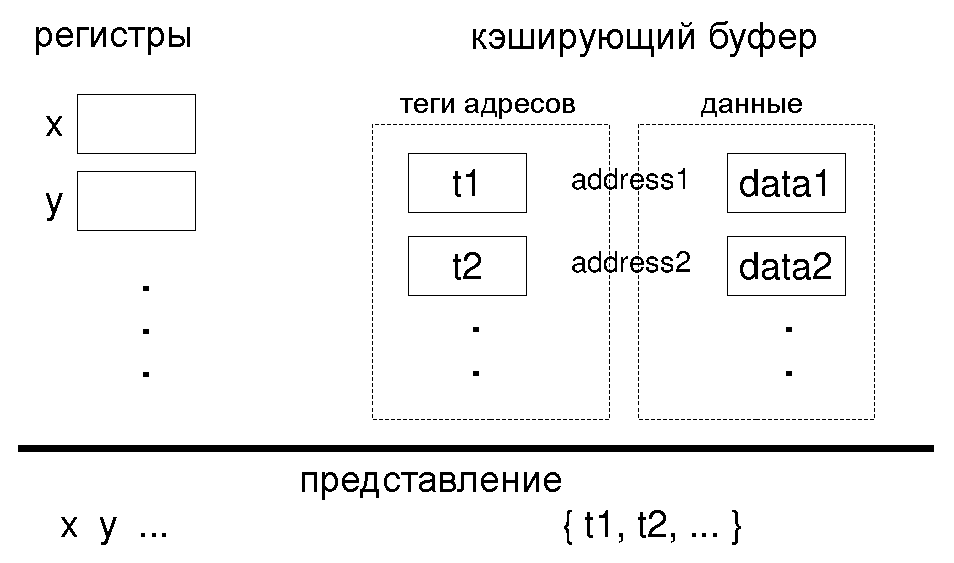
\includegraphics[width=0.5\textwidth]{2.theor/mpset}\\
  \caption{Представление состояния микропроцессора}\label{mpset}
\end{figure}

Ограничения для тестовых ситуаций в кэширующих буферах могут
включать адреса, с которыми работает инструкции.

\begin{utv}\label{hit_miss_simpleform}
Тестовые ситуации в кэширующих буферах имеют следующую простую форму
с использованием переменных $L$ -- текущее состояние (содержимое)
кэширующего буфера (множество тегов данных), $x$ -- тег адреса
данных в инструкции):
\begin{itemize}
\item \emph{кэш-попадание} выражается в виде ограничения $x \in L$;
\item \emph{кэш-промах} выражается в виде ограничения $x \notin L$.
\end{itemize}
\end{utv}

Для переменной $L$ в каждой инструкции методом индукции может быть
составлено следующее выражение. База: $L$ для первой инструкции есть
начальное содержимое кэширующего буфера, это переменная величина в
системе уравнений. Теперь индуктивный шаг. Пусть выражение для
очередной инструкции $L$, а для следующей -- $L'$. Тогда если
тестовая ситуация очередной инструкции -- кэш-попадание, то $L'
\equiv L$ (так как содержимое не меняется), а если кэш-промах с
адресом $x$, то $L' \equiv (L \setminus \{x'\} \cup \{x\})$ (так как
в кэширующий буфер при промахе добавляются данные по нужному адресу,
а некоторые данные вытесняются, $x'$ есть адрес вытесняемых данных).
Для новой переменной $x'$ добавим в систему такие уравнения: $x' \in
L \wedge displaced(x') \wedge R(x) = R(x')$, предикат
$displaced(x')$ истинен, если $x'$ является адресом вытесняемых
данных в данной инструкции. Предикат $displaced$ описывает
\emph{стратегию вытеснения}, т.е. правило, по которому в кэширующем
буфере выбираются данные, которые следует удалить (вместе с тегом),
а на их место поместить данные, вызвавшие промах. Для кэширующего
буфера прямого отображения общезначимо утверждение $(R(x) = R(x'))
\rightarrow displaced(x')$, поэтому для такого типа кэширующих
буферов уравнение $displaced(x')$ можно исключить из ограничений.
Функциональный символ $R$ используется для задания набора, которому
относится адрес, в кэширующих буферах прямого отображения и
наборно-ассоциативных кэширующих буферах. Возможна такая семантика
этого символа -- $R(x)$ это множество адресов, которые потенциально
могут находиться в том же наборе, что и набор адреса $x$ (верно
утверждение, что адрес не может соответствовать более чем одному
набору и не соответствовать никакому набору вообще, одному набору
могут соответствовать разные адреса). Или такая семантика -- $R(x)$
это номер набора адреса $x$. Для составления уравнений может быть
выбрана любая семантика. Для полностью-ассоциативных кэширующих
буферов уравнение $R(x) = R(x')$ является тождественной истиной,
поскольку в нем все адреса соответствуют одному набору.

Следующая теорема описывает выражение для $L$ без использования
индукции и способ составления ограничений для тестовых ситуаций в
кэширующих буферах:
\begin{lemma}\label{L_current} \LcurrentBody
\end{lemma}
Доказательство леммы приведено в приложении~\ref{proofs}.

Например, если перед данной инструкцией располагается 3 инструкции с
кэш-промахом, то $L \equiv L_0 \setminus \{x'_1, x'_2, x'_3\} \cup
(\{x_1\} \setminus \{x'_2, x'_3\}) \cup (\{x_2\} \setminus \{x'_3\})
\cup \{x_3\}$.

\begin{theorem}[Дизъюнктивная форма уравнений для тестовых ситуаций
в кэширующих буферах]\label{hit_miss_equations} \HitMissEquations
\end{theorem}
\begin{proof}
Применим утверждение~\ref{hit_miss_simpleform} для представления
тестовой ситуации и лемму~\ref{L_current} для записи текущего
состояния кэширующего буфера. Для вытесняемого тега записываем те же
ограничения, что и для кэш-попадания, поскольку вытесняемый тег
принадлежит текущему состоянию кэширующего буфера. Кроме того для
вытесняемого тега формулируются дополнительные ограничения --
$displaced(x')$ (стратегия вытеснения) и $R(x) = R(x')$ (из
определения вытеснения: вытесняемый тег обязательно относится к тому
же региону, что и вытесняющий).
\end{proof}

Заметьте, что получившиеся ограничения для кэш-попадания и
кэш-промаха получились очень похожими, хотя изначально у них было
два совершенно противоположных представления.

Теорему~\ref{hit_miss_equations} можно переформулировать без
использования вытеснямых тегов:

\begin{utv}\label{hit_miss_human} Пусть $L_0$ -- множество
адресов данных, расположенных в кэширующем буфере перед исполнением
первой инструкции тестового шаблона. Тогда
\begin{itemize}
\item для инструкции с кэш-попаданием адреса $x$ следует добавить
следующую совокупность уравнений:
$$
\left[
   \begin{array}{l}
    x \in L_0 \wedge x~\mbox{все еще не вытеснен} \\
    x~\mbox{внесен одним из кэш-промахов} \wedge \mbox{с тех пор не вытеснен} \\
   \end{array}
  \right.
$$

\item для инструкции с кэш-промахом адреса $x$ следует добавить следующую систему
уравнений ($\{x_i\}$ -- множество адресов данных в инструкциях с
кэш-промахами, расположенными до текущей инструкции):
$$
\left[
   \begin{array}{l}
    x \notin L_0 \wedge x \notin \{x_1, x_2, ..., x_n\} \\
    x~\mbox{был вытеснен} \wedge \mbox{не был больше внесен в буфер}\\
  \end{array}
\right.
$$

\end{itemize}
\end{utv}

Формально показано, что утверждение~\ref{hit_miss_human} описывает
все возможные сценарии появления и вытеснения данных в кэширующих
буферах. Однако применение этих ограничений в данном виде для
реальных микропроцессоров может быть ограничено из-за большого
размера $L_0$ (что влечет к большому размеру ограничений и к
невозможности разрешения таких больших ограничений доступными
инструментами). Далее будет показано, как \emph{совместное
рассмотрение} тестовых ситуаций разных буферов и таблиц позволят
существенно сократить размер этой формулы и обратиться к генерации
ограничений для описания вытеснения.

\section{Совместная генерация ограничений}

В этом разделе формально ставится задача генерации тестовых данных
для последовательности тестовых ситуаций в кэширующем буфере,
выделяется подзадача описания механизма вытеснения и описывается
метод построения ограничений обозримого размера для генерации
тестовых программ по тестовым шаблонам с использованием ограничений.
Идея совместного метода заключается в использовании содержимого
нескольких кэширующих буферов и таблиц одновременно.



\subsection{Особенности исполнения инструкций обращения к памяти
на современных микропроцессорах}

В инструкции обращения к памяти в современных микропроцессорах
задействована не одна подсистема. Исполнение инструкции обращения к
памяти можно разбить на два этапа -- подготовка физического адреса и
собственно обращение с памятью (см.рис.~\ref{memoryAccess}).

\begin{figure}[h] \center
  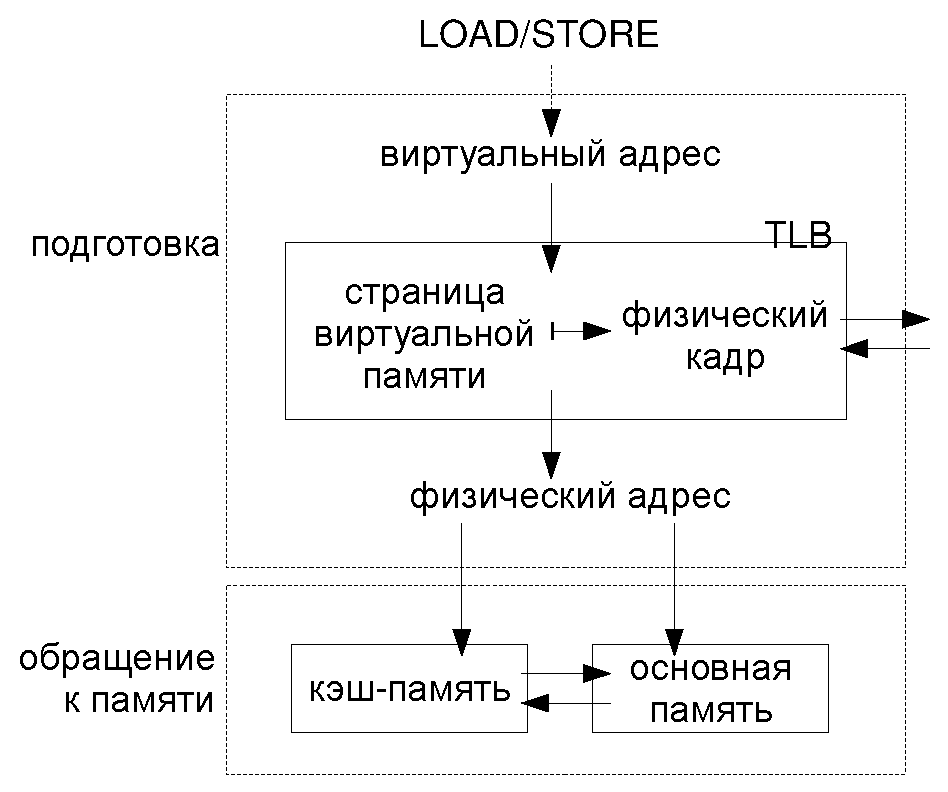
\includegraphics[width=0.5\textwidth]{2.theor/instr}\\
  \caption{Модель исполнения инструкции обращения к памяти}\label{memoryAccess}
\end{figure}

Подготовка физического адреса включает в себя формирование
\emph{виртуального адреса данных}, с которыми необходимо выполнить
операцию (некоторые архитектуры сначала вычисляется
\emph{эффективный адрес}~\cite{PowerPC750}, затем на его основе
виртуальный, а на его основе физический). Виртуальный адрес
формируется на основе аргументов инструкции. Формирование
физического адреса на основе виртуального адреса производится с
использованием TLB. По сути по виртуальному адресу вычисляется номер
страницы виртуальной памяти и смещение внутри этой страницы
(зачастую это битовые поля виртуального адреса), для страницы
виртуальной памяти выбирается соответствующий физический кадр,
используя TLB, и, наконец, физический адрес составляется из
полученного номера физического кадра и смещения внутри страницы (оно
берется из виртуального адреса). TLB содержит некоторое количество
пар, задающих соответствие номера страницы виртуальной памяти и
номера физического кадра. Размер самой страницы в виртуальной памяти
и физической памяти совпадает, поэтому смещение внутри страницы
используется в физическом адресе без изменений по сравнению с
виртуальным адресом.

Когда физический адрес готов, осуществляется обращение к памяти:
загрузка данных из памяти или сохранение данных в памяти. При этом
если данные по физическому адресу имеются в кэш-памяти, основная
память может остаться неизменной. Это сделано для повышения
эффективности работы с основной памятью.

%//////////////TODO зачем нужно было применять такие сложные вещи? может быть,
%20\% труда сделает 80\% работы (обычным рандомом), а в оставшемся
%небольшом остатке работы надо действовать более интеллектуально (а
%если вероятность (отношение количества тестовых данных к количеству
%значений в их области определения) не мала, то прагматический вопрос
%стоит очень остро); другой момент - \textbf{у Genesys-Pro очень
%много положительных моментов} и самый главный -- масштабируемость,
%напротив моё решение плохо масштабируемо, значит, надо искать
%критерий, по которому мое решение лучше... Если бы не цена
%Genesys-Pro, стоило ли делать эту работу?

%\subsection{Уровни генерации тестовых данных}
%
%Тестовая программа некоторым специальным образом меняет состояние
%микропроцессора. Однако для того, чтобы это исполнение было
%согласовано с тестовым шаблоном, необходимо перед исполнением
%инструкций тестового шаблона перевести микропроцессор в некоторое
%специальное состояние (изменить значения в регистрах, в ячейках
%кэширующих буферов, возможно в ячейках оперативной памяти). Обычно
%изменение значения в регистре выполняется одной инструкцией, которая
%не затрагивает остальные компоненты микропроцессора. Таким образом,
%изменение значений в регистрах можно проводить последовательностью
%инструкций, каждая из которых меняет один регистр. Значения, которые
%надо поместить в регистры, входят в модель ограничений, генерируемых
%по тестовому шаблону. Однако изменение кэширующих буферов не всегда
%возможно выполнять независимо от остальных кэширующих буферов (в
%качестве примера можно привести кэш-память первого и второго
%уровней, которые могут измениться совместно).
%
%Поэтому задача построения тестовой программы для тестового шаблона
%может быть поделена на подзадачи в зависимости от того, состояние
%каких кэширующих буферов разрешается изменять перед исполнением
%инструкций тестового шаблона. От этого в том числе будет зависеть и
%выбор переменных для ограничений (\emph{тестовых данных}). Задача
%вычисления значений этих переменных называется задачей
%\emph{генерации тестовых данных}. Она может быть представлена в
%следующих формах:
%\begin{itemize}
%\item \emph{простая форма:} найти начальное состояние
%микропроцессора (тестовыми данными являются содержимое кэширующих
%буферов, таблиц и значения регистров); построение инструкций,
%приводящих кэширующие буферы и таблицы в это состояние, не входит в
%ограничения и должно выполняться после разрешения ограничений (т.е.
%получения тестовых данных); иными словами, результатом разрешения
%ограничений являются значения в ячейках буферов и таблиц, а
%инструкции, которые поместят эти значения в буферы и таблицы, должны
%быть получены иными алгоритмами~\cite{my_programmirovanie_2009}; при
%выполнении тестовой программы сгенерированные инструкции
%инициализации микропроцессора могут быть исполнены некорректно и
%тогда на инструкциях тестового шаблона могут не проявиться
%действительные ошибки или появиться ложные ошибки;
%\item \emph{минимальная форма:} найти лишь значения регистров, используя
%данное начальное состояние (содержимое) кэширующих буферов и таблиц
%(тестовыми данными являются только значения регистров); инструкции,
%подготавливающие состояние микропроцессора, не меняют кэширующие
%буферы и таблицы, что повышает качество тестирования, однако в такой
%форме задача генерации тестовых данных может быть неразрешима (при
%разрешимой другой форме), т.е. тестовая программа с таким
%дополнительным ограничением не будет существовать, хотя без него
%будет;
%\item \emph{смешанная форма:} требуется построить
%значения регистров и последовательность инструкций инициализации
%состояния микропроцессора (тестовыми данными являются значения
%регистров и аргументы инструкций инициализации); эта форма является
%компромиссом между простой и минимальной формой, правда в такой
%форме увеличивается сложность задачи построения и разрешения
%ограничений, потому что невозможно заранее предугадать, сколько
%необходимо и достаточно дополнительных инструкций.
%\end{itemize}
%
%Задачу поиска тестовых данных в минимальной форме будем называть
%задачей генерации тестовых данных \emph{нулевого уровня}. Дальнейшие
%уровни определяются возможностью изменять кэширующие буферы и
%таблицы разными инструкциями. Например, для архитектуры
%MIPS~\cite{mips64_II} были выделены следующие уровни генерации
%тестовых данных помимо нулевого уровня:
%\begin{itemize}
%\item на \emph{первом уровне} разрешается менять те строки TLB,
%которые не находятся в буфере TLB; изменение одной строки можно
%делать независимо от остальных строк и буфера одной инструкцией
%(TLBWI);
%\item на \emph{втором уровне} разрешается менять любую строку TLB;
%при этом кроме смены строк, не входящих в буфер TLB, нужно
%переинициализировать содержимое буфера (на каждую строку отдельная
%инструкция);
%\item на \emph{третьем уровне} разрешается менять и TLB, и кэш-память.
%\end{itemize}
%
%Чем больше уровень, тем длиннее будет инициализирующая программа и
%тем сложнее ее построить.

\subsection{Выделение подзадач на кэширующие буферы}\label{module_algorithm}

Каждая инструкция может быть снабжена набором атрибутов, отвечающих
отдельным этапам исполнения инструкции: аргументы, виртуальные
адреса, физические адреса, теги, данные для обращения к памяти.
Поскольку ограничения, описывающие в явном виде изменение состояния
кэширующих буферов и таблиц в результате исполнения инструкций
(инструкция представлена набором значений атрибутов, состояние
кэширующих буферов и таблиц множеством значений ячеек), получаются
очень большого размера (порядка $|L| \cdot 2^n$, где $|L|$ -- размер
состояния кэширующего буфера, $n$ -- количество инструкций), то было
принято решение использовать \emph{неявное} задание инструкции. А
именно, строить ограничения только на атрибутах всех инструкций.
Ограничения на атрибуты одинаковой семантики выделим в отдельные
\emph{подзадачи}. Среди таких подзадач будут \emph{подзадачи на
кэширующие буферы}. Например, это могут быть подзадачи на описание
физических адресов инструкций на основе тестовых ситуаций на
кэш-память.

Везде далее под формулировкой тестового шаблона как
последовательности пар $(S_i, x_i)$ будет пониматься именно
подзадача на некоторый кэширующий буфер. Последовательность $(S_i)$
задает последовательность тестовых ситуаций на этот кэширующий
буфер, а $(x_i)$ -- последовательность тегов.

Если имеется несколько подзадач, то конъюнкция их ограничений может
иметь существенно меньший размер, чем размер самих ограничений для
отдельных подзадач. На этой идее и основан \emph{метод совместной
генерации ограничений}.

Отдельно рассмотрим часто встречающуюся \emph{задачу на основную
память}. Она задает соответствие между значениями регистров,
физическими адресами и значениями ячеек оперативной памяти. Если
представить основную память в виде одномерного массива $memory$,
индексация в котором идет по физическим адресам, то:
\begin{itemize}
\item инструкцию, осуществляющую загрузку из памяти,
можно представлять как $R := memory[physicalAddress]$;
\item инструкцию, осуществляющую сохранение в памяти,
можно представлять как $memory[physicalAddress] := R$.
\end{itemize}
Таким образом, получается последовательность присваиваний, которая
может быть преобразована в систему уравнений с помощью
\emph{редукции Аккермана} (или
\emph{аккерманизации})~\cite{Ackermann}. А именно,
\begin{itemize}
\item для каждой упорядоченной пары инструкций (не обязательно
находящиеся подряд в тестовом шаблоне, но в том же порядке)\\
$STORE(R_1, p_1)$ и $LOAD(R_2, p_2)$ создается ограничение $$ (p_1 =
p_2 \wedge p_2 \notin \{ p_{(1)}, p_{(2)}, ..., p_{(k)}\})
\rightarrow R_1 = R_2$$ где $p_{(1)}, p_{(2)}, ..., p_{(k)}$ --
физические адреса инструкций $STORE$, расположенных между двумя
инструкциями этой пары;
\item для каждой упорядоченной пары инструкций (не обязательно
находящиеся подряд в тестовом шаблоне, но в том же порядке)\\
$LOAD(R_1, p_1)$ и $LOAD(R_2, p_2)$ создается ограничение $$ (p_1 =
p_2 \wedge p_2 \notin \{ p_{(1)}, p_{(2)}, ..., p_{(k)}\})
\rightarrow R_1 = R_2$$ где $p_{(1)}, p_{(2)}, ..., p_{(k)}$ --
физические адреса инструкций $STORE$, расположенных между двумя
инструкциями этой пары.
\end{itemize}

\subsection{Метод совместной генерации ограничений}

Введем понятие <<тегсет>> и с помощью него выразим тестовые ситуации
в кэширующих буферах. Обращение к кэширующему буферу по данному
адресу осуществляется на основе тега и индекса, которые вычисляются
на основе адреса. По индексу из всех секций кэширующего буфера
выбираются пары <<(тег, значение)>>. Далее осуществляется поиск тега
адреса среди тегов выбранных пар. Зачастую тег адреса и индекс
адреса вычисляются как битовые поля адреса. Битовую конкатенацию
тега и индекса будем называть \emph{тегсетом} адреса. Если
кэширующий буфер является полностью ассоциативным, то тегсет
совпадает с тегом адреса.

\begin{figure}[h] \center
  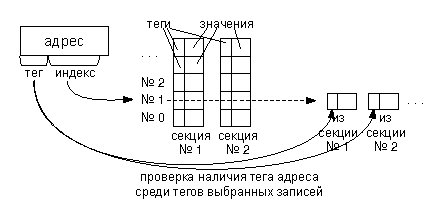
\includegraphics[width=0.8\textwidth]{2.theor/cache_operation}\\
  \caption{Тег и индекс адреса}\label{cache_operation}
\end{figure}

В микропроцессорах зачастую тегсет является инвариантом при
обращениях в разные уровни кэш-памяти (обычно это делается для того,
чтобы не менялись оставшиеся биты физического адреса, они задают
смещение в строке кэш-памяти, и постоянство этих бит позволяет легко
перемещать строки кэш-памяти между разными уровнями).

\begin{figure}[h] \center
  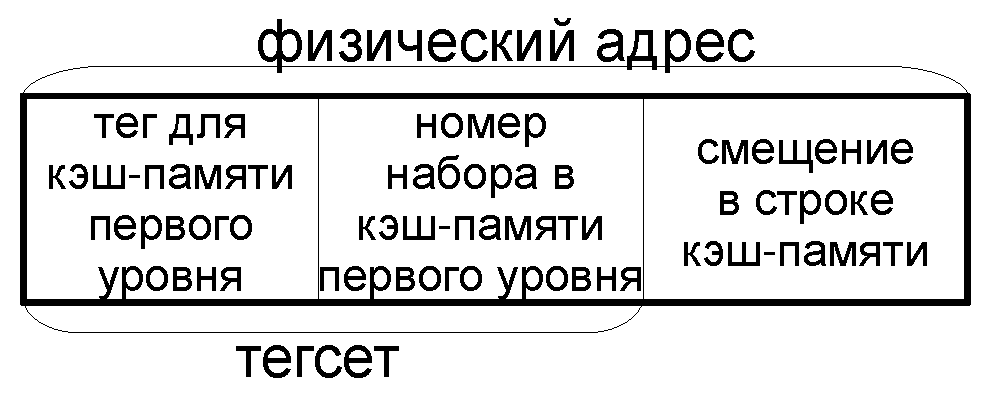
\includegraphics[width=0.5\textwidth]{2.theor/tagset}\\
  \caption{Тегсет физического адреса}\label{tagset}
\end{figure}

Тегсеты могут быть использованы для представления тестовых ситуаций
в кэширующих буферах с использованием ограничений таким же образом,
как это делалось для тегов: $x \in L$ для кэш-попадания и $x \notin
L$ для кэш-промаха, где $x$ -- тегсет адреса, а $L$ -- множество
тегсетов данных, хранящихся в кэширующем буфере перед исполнением
инструкции. Множество тегсетов составляется битовой конкатенацией
тега и индекса в каждом элементе начального содержимого кэширующего
буфера. Для тегсетов аналогичным образом формулируются и
доказываются лемма~\ref{L_current} и
теорема~\ref{hit_miss_equations} об ограничениях для тестовых
ситуаций в кэширующих буферах, сформулированных уже на тегсетах.

Рассмотрим следующее представление тестового шаблона, которое
назовем \emph{схемой последовательностей тестовых ситуаций}. По
одной оси будут располагаться инструкции тестового шаблона, по
другой оси -- кэширующие буферы микропроцессора
(см.рис.~\ref{template_scheme}). На пересечении инструкции и буфера
будет помещаться переменная -- тег или тегсет, если для этой
инструкции в тестовом шаблоне есть тестовая ситуация на обращение в
этот кэширующий буфер. Будем считать, что в исполнении инструкции
задействованы те кэширующие буферы, тестовые ситуации на которые
указаны в тестовом шаблоне для этой инструкции. Схема
последовательностей тестовых ситуаций позволяет увидеть имеющиеся в
тестовом шаблоне \emph{совместные} обращения в кэширующие буферы,
увидеть последовательности обращений к отдельным буферам, таким
образом оценить сложность будущих ограничений.

\begin{figure}[h] \center
  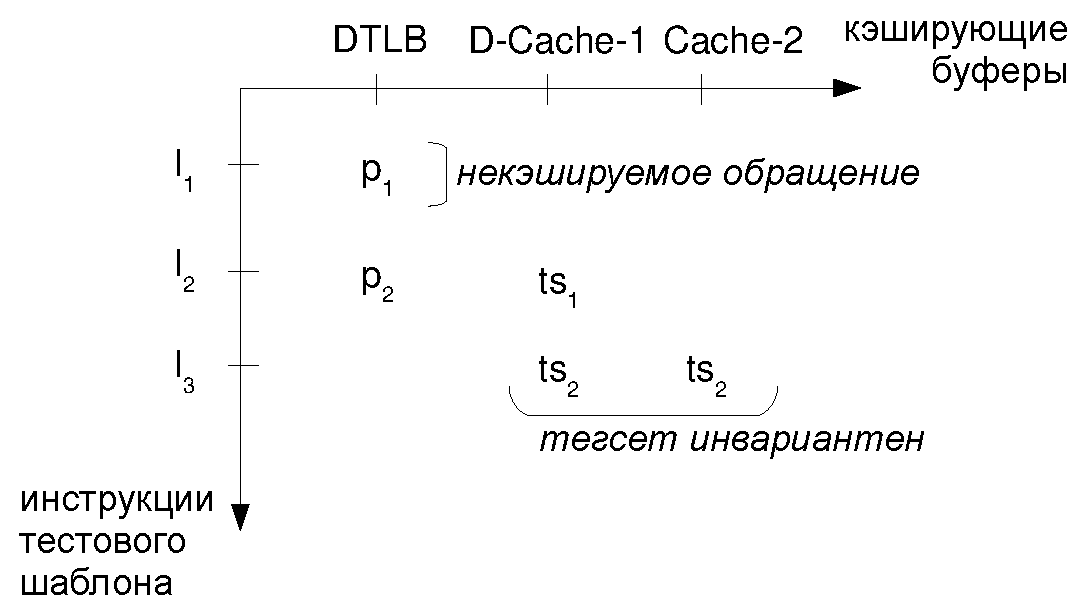
\includegraphics[width=0.6\textwidth]{2.theor/template_scheme}\\
  \caption{Пример схемы последовательностей тестовых ситуаций}\label{template_scheme}
\end{figure}

Для каждой последовательности тестовых ситуаций вводятся
переменные-теги или тегсеты, а генерируемые для тестового шаблона
ограничения состоят из ограничений для каждой такой переменной и
ограничения, описывающие отношения введенных переменных. Этот
процесс можно выразить следующей последовательностью шагов:
\begin{enumerate}
  \item составить модель MMU (выделить кэширующие буферы и
  таблицы);
  \item выделить последовательности тестовых ситуаций в тестовом
  шаблоне (составить \emph{схему последовательностей тестовых
  ситуаций});
  \item ввести переменные-теги тестовых ситуаций; если
  возможно, уменьшить количество переменных, заменив некоторые теги
  на тегсеты;
  \item выделить последовательности тестовых ситуаций, для записи
  которых потребуются большие массивы данных;
  \item построить ограничения для каждого тегсета -- при обращении к
  большим массивам данных строить \emph{совместные ограничения}.
\end{enumerate}

Последний шаг требует пояснения. Пусть имеются две тестовые ситуации
на кэширующие буферы. Упорядочим их в таком порядке, что данные,
полученные из первого буфера, связаны с тегом обращения ко второму
кэширующему буферу (см.рис.~\ref{conjunctive}). Причем первый
кэширующий буфер подчинен некоторой таблице.

\begin{figure}[h] \center
  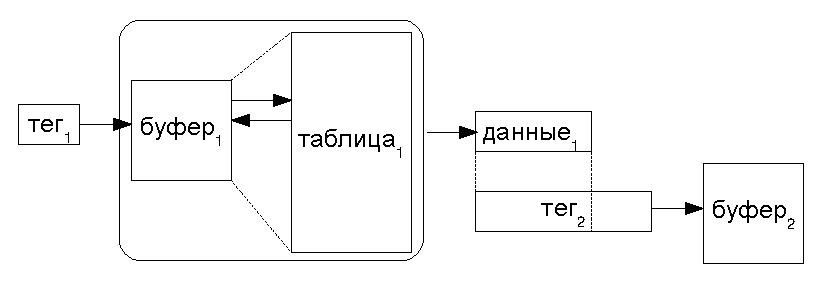
\includegraphics[width=0.6\textwidth]{2.theor/conjunctive}\\
  \caption{Совместные обращения в буферы}\label{conjunctive}
\end{figure}

В ограничениях появляется содержимое буферов целиком (иначе можно
просто выписать ограничения на первый и на второй буфер без
изменения). Согласно теореме~\ref{hit_miss_equations} для
кэш-попадания в первом буфере можно записать ограничения:
$$
\left[\begin{array}{l} t_1 \in T_1 \wedge \mbox{...}\\
t_1 = t_2 \wedge \mbox{...}
\end{array}\right.
$$

Значит, при этом тег принадлежит либо множеству тегов первого
буфера, либо множеству тегов из таблицы, которой подчинен первый
буфер. Из этого следует, что данные -- результат обращения в первый
буфер -- либо принадлежат данным из буфера ($TD_1$), либо
принадлежат данные из таблицы ($FD_1$). Для кэш-промаха ограничения:

$$
\left[\begin{array}{l} t_1 \notin T_1 \wedge \mbox{...}\\
t_1 = t_2' \wedge \mbox{...}
\end{array}\right.
$$

Соответственно, либо тег не принадлежит множеству тегов первого
буфера, но принадлежит множеству тегов в таблице, которой подчинен
первый буфер, либо тег принадлежит тегам той же таблицы (т.к. этим
тегам принадлежит $t_2'$). Значит, при кэш-промахе данные,
получаемые после обращения в первый кэширующий буфер, либо
принадлежат $FD_1 \setminus TD_1$, либо принадлежат $FD_1$.

Далее, учтем, что биты данных, полученных из первого буфера, связаны
с битами тега для обращения во второй буфер. Для обращения во второй
кэширующий буфер снова выпишем ограничения, согласно
теореме~\ref{hit_miss_equations}. Для кэш-попадания в одну из
конъюнкций входит большой массив тегов второго буфера:

$$
\left[\begin{array}{l} x_1 \in X_1 \wedge \mbox{...}\\
x_1 = x_2 \wedge \mbox{...}
\end{array}\right.
$$

Но поскольку тег связан с данными, полученными из первого буфера,
конъюнкция ограничений позволяет сократить множество тегов $L$,
оставив только те, которые подходят под множество констант,
участвующих в ограничении для обращения в первый буфер. Например,
вместо ограничения $x \in L$ если данные из первого буфера $d$
являются битовым полем $x$ (например, номер физического кадра
является битовым полем тегсета при обращении в кэш-память) и $d \in
DD$ можно записать ограничение $x \in L \cap [DD]$, т.е. $x \in
\{\lambda | \lambda \in L \wedge \lambda_{\mbox{биты данных}} \in
DD\}$. Соответствующее упрощение можно сделать и для $d$: $d \in
\widehat{L \cap [DD]}$, т.е. $d \in \{\delta | \delta \in DD \wedge
\exists x \in L : \delta = x_{\mbox{биты данных}}\}$. Множества
констант $L \cap [DD]$ и $\widehat{L \cap [DD]}$ могут быть
вычислены до генерации ограничений. Обычно множество $L \cap [DD]$
имеет значительно меньший размер, чем $L$, что позволяет существенно
сократить размер ограничений. В этом и заключается основной эффект
применения совместной генерации ограничений. Для кэш-промаха
получаются похожие ограничения, только вместо $x \notin L$ будет $x
\notin L \cap [DD]$.

Надо быть аккуратным, ведь не всегда таблицы и буферы имеют
действительно большой размер и иногда множество тегов, которое
входит в ограничения, может быть выписано целиком. Например, при
рассмотрении конъюнкции следующих подформул (первая получена от
кэш-попадания в кэш-памяти по тегу $x$, вторая получена от тестовой
ситуации в TLB, $\hat{x}$ -- номер физического кадра, входящий в
$x$):

$$
\left\{\begin{array}{l} x = x_i \wedge \mbox{...}\\
\hat{x} \in PFN \wedge \mbox{...}
\end{array}\right.
$$

искать множество $L$ и пересекать его с $PFN$ не нужно, потому как
$PFN$ небольшого размера выписывается целиком (а большого размера и
не участвует в ограничения -- см.теорему~\ref{hit_miss_equations}).



%Выражение -- множество констант -- в совместном ограничении на
%тегсет будем называть \emph{доменом} тегсета. С использованием этого
%определения сформулируем вариант теоремы~\ref{hit_miss_equations}
%для совместной генерации ограничений:
%
%\begin{utv}\label{hit_miss_human_domain} Пусть $D$ -- домен
%тегсета адреса $x$ текущей инструкции. Тогда
%\begin{itemize}
%\item если тестовая ситуация текущей инструкции -- кэш-попадание, то следует добавить
%следующую совокупность уравнений:
%$$
%\left[
%   \begin{array}{l}
%    x \in D \wedge x~\mbox{все еще не вытеснен} \\
%    x~\mbox{внесен одним из кэш-промахов} \wedge \mbox{с тех пор не вытеснен} \\
%   \end{array}
%  \right.
%$$
%
%\item если тестовая ситуация текущей инструкции -- кэш-промах, то следует добавить
%следующую совокупность уравнений ($\{x_i\}$ -- множество тегсетов
%предыдущих инструкций с кэш-промахами):
%$$
%\left[
%   \begin{array}{l}
%    x \notin D \wedge x \notin \{x_1, x_2, ..., x_n\} \\
%    x~\mbox{был внесен} \wedge x~\mbox{был затем вытеснен} \wedge \mbox{не был больше внесен в
%    кэш-память}\\
%    x \in D \wedge x~\mbox{был вытеснен} \wedge \mbox{не был больше внесен в
%    кэш-память}\\
%  \end{array}
%\right.
%$$
%
%\end{itemize}
%\end{utv}
%
%В заключение назову границы применимости совместной генерации
%ограничений. Начальное состояние кэш-памяти и TLB может быть
%использовано целиком для генерации тестовых данных нулевого уровня.
%Но для более высоких уровней надо применять более изощренные
%алгоритмы (например, вводить некую небольшую область в кэш-памяти и
%TLB, представлять ее переменными величинами, включать в ограничения,
%результатом разрешения этих ограничений будет инициализация этой
%неизвестной части). Другим важным требованием совместной генерации
%является \emph{существенность} совместного исполнения инструкции,
%иными словами, инструкция должна задействовать и кэш-память, и TLB
%(это может управляться сегментом виртуального адреса -- для
%трансляции виртуальных адресов из некоторых сегментов может не
%использоваться TLB, а обращение в память по физическим адресам,
%полученным из некоторых строк TLB, может происходить без участия
%кэш-памяти). В случае неотображаемого кэшируемого обращения (TLB не
%задействован, кэш-память задействована) нет возможности построить
%более компактную конъюнкцию.
%
%Однако несмотря на приведенные ограничения, метод совместной
%генерации ограничений можно рассматривать как быстрый
%\emph{достаточный} алгоритм решения задачи построения тестовых
%данных (не являющийся необходимым). И если он не дал решение, то
%воспользоваться уже другими более продвинутыми методами генерации
%тестовых данных.

\subsection{Корректность и условная полнота совместной генерации}

\begin{theorem}[Корректность метода совместной генерации
ограничений] Если ограничения, сгенерированные для некоторого
тестового шаблона методов совместной генерации, совместны и дают в
качестве решения начальные значения регистров
$r_1,~r_2,~\dots,~r_R$, то для этого тестового шаблона существует
тестовая программа, инициализирующая часть которой содержит лишь
загрузку в регистры значений $r_1,~r_2,~\dots,~r_R$.
\end{theorem}
\begin{proof}
  Ограничения, которые построены методом совместной генерации,
  отличаются от определений тестовых ситуаций лишь эквивалентной
  записью конъюнкции ограничений с множеством значений. Если
  переменные удовлетворяют конъюнкции, то они удовлетворяют каждому
  элементу этой конъюнкции, т.е. тестовая программа, составленная с
  ними, будет соответствовать тестовому шаблону.
\end{proof}

\begin{theorem}[Условная полнота метода совместной генерации ограничений]
Пусть выбран некоторый тестовый шаблон, в котором все обращения в
кэширующие буферы являются совместными. Тогда если для него
существует тестовая программа, в инициализирующей части которой не
меняется состояние кэширующих буферов, то ограничения, составленные
методов совместной генерации, будут совместны.
\end{theorem}
\begin{proof}
  Ограничения, которые построены методом совместной генерации,
  отличаются от определений тестовых ситуаций лишь эквивалентной
  записью конъюнкции ограничений с множеством значений. Если
  переменные удовлетворяют каждому элементу конъюнкции (а это верно,
  поскольку существует тестовая программа), то они удовлетворяют и
  конъюнкции, что и означает совместность искомой системы ограничений.
\end{proof}

%%%%%%%%%%%%%%%%%%%%%%%%%%%%%%%%%%%%%%%%%%%%%%%%%%%%%%%%%%%%%%%%%%%%

%\pagebreak
\section{Зеркальная генерация тестовых данных}

Метод совместной генерации ограничений позволяет эффективно
построить тестовую программу, если для каждой инструкции имеется
более одного задействовано кэширующего буфера. Однако возможны
случаи, например, неотображаемого кэшируемого обращения в
микропроцессоре с TLB и кэш-памятью большого размера, когда в
ограничениях, генерируемых согласно
теореме~\ref{hit_miss_equations}, невозможно уменьшить размер $L_0$.

Другой случай -- это так называемая \emph{VIVT кэш-память}
(virtually indexed virtually tagged)~\cite{HennessyPatterson3rd}. В
этой кэш-памяти данные снабжены тегами виртуального адреса (в
virtually indexed physically tagged кэш-памяти данные снабжены
тегами физического адреса). Такая кэш-память в основном применяется
для кэширования инструкций. Эта кэш-память характеризуется тем, что
обращение к кэш-памяти первого уровня не требует предварительной
трансляции виртуального адреса в физический. Однако ограничения,
генерируемые согласно теореме~\ref{hit_miss_equations}, для
кэш-попадания нет возможности выделить совместное обращение (для
кэш-промаха совместное обращение возможно).

Противоположный случай -- когда составить систему ограничений
методом совместной генерации можно, но эта система оказывается
несовместной.

Однако если архитектура микропроцессора позволяет изменять
кэширующие буферы с помощью отдельных инструкций (возможно, при
особом значении некоторых регистров микропроцессора или области
виртуальной памяти), то можно воспользоваться этими инструкциями для
добавления в кэширующий буфер данных по тем тегам, которые будут
использованы в тестовой программе (а их уже можно выбирать
произвольно, что сильно упростит систему ограничений). При этом
можно не задумываться над тем, были ли эти теги в $L_0$ или нет.
Иными словами, если обращение к кэширующему буферу по некоторому
тегу должно быть успешным, то перед этим обращением должно быть
другое обращение по этому же тегу, после которого данные по этому
тегу не вытесняются до нужного обращения. Дополнительных
ограничений, кроме уже упомянутых, на тег не накладывается. Если
обращение к кэширующему буферу по некоторому тегу должно быть
неуспешным, то перед этим обращением всё равно должно быть другое
обращение по этому же тегу, после которого однако данные по этому
тегу должны быть вытеснены и не положены вновь до нужного обращения.
Таким образом, у каждого тега в тестового шаблона есть свой
<<зеркальный>> тег среди предыдущих тегов тестового шаблона или
дополнительных тегов инициализирующей программы.

Более формально, для данной последовательности тестовых ситуаций для
кэширующего буфера $(S_i, x_i)$, где $i = 1, 2, ..., n$, $S_i$ --
hit или miss, $x_i$ -- тег данных, требуется построить
последовательность тегов $t_j$ (\emph{инициализирующая
последовательность тегов}), $j = 1, 2, ..., m$, которые обеспечивают
данную последовательность тестовых ситуаций. Согласно зеркальному
методу для каждого данного тега $x_i$ при $S_i = $ hit надо
составить систему уравнений
$$
\left\{\begin{array}{l} x_i \in \{t_1, ..., t_m, x_1, ...,
x_{i-1}\}\\
x~\mbox{не вытеснен с момента последнего к нему}\\
\mbox{\quad обращения в}~t_1, ..., t_m, x_1, ..., x_{i-1}
\end{array} \right.
$$

а при $S_i = $ miss надо составить систему уравнений

$$
\left\{\begin{array}{l} x_i \in \{t_1, ..., t_m, x_1, ...,
x_{i-1}\}\\
x~\mbox{вытеснен и не добавлен с момента последнего}\\
\mbox{\quad к нему обращения в }~t_1, ..., t_m, x_1, ..., x_{i-1}
\end{array} \right.
$$

\begin{lemma}\label{monotonic_m}Если существует решение для некоторого $m$, то
существует решение и для $m+1$.
\end{lemma}
\begin{proof}
  Достаточно взять $t_{m+1} = t_m$.
\end{proof}

Ниже будет показано, что достаточно рассматривать $m$, ограниченные
линейной функцией от $n$ и $w$ (ассоциативности кэширующего буфера).
Поэтому может быть поставлена задача минимизации параметра $m$
(длины инициализирующей программы). Это увеличит качество
тестирования, поскольку уменьшит влияние дополнительных,
инициализирующих, инструкций на исполнение инструкций тестового
шаблона. Минимизация может быть эффективно выполнена с
использованием двоичного поиска оптимального значения $m$
(лемма~\ref{monotonic_m} показывает корректность применения
двоичного поиска) -- границу сверху для значения $m$ дает
теорема~\ref{mirror_fullness}.

\begin{utv}[Применимость зеркального метода]
Зеркальный метод генерации ограничений применим к данному тестовому
шаблону для данной архитектуры микропроцессоров, если система команд
микропроцессора содержит инструкции, позволяющие (при определенных
условиях) изменение задействованных в тестовом шаблоне кэширующих
буферов по отдельности от остальных кэширующих буферов.
\end{utv}

Например, в архитектуре MIPS~\cite{mips64_II} инструкции обращения к
памяти могут быть исполнены:
\begin{itemize}
  \item в некэширующем отображаемом режиме -- это позволяет изменять
  буфер данных TLB отдельно от кэш-памяти;
  \item в кэшируемом неотображаемом режиме -- это позволяет изменять
  кэш-память данных отдельно от буфера данных TLB.
\end{itemize}

При этом инструкции могут быть исполнены в кэшируемом или
отображаемом режиме по отношению к кэш-памяти инструкций или буферу
инструкций TLB. Для возможности применения зеркального метода в
случае, когда тестовый шаблон содержит тестовые ситуации на
кэш-память данных и на кэш-память инструкций, надо выбирать
расположение инициализирующих инструкций в памяти так, чтобы при
исполнении каждой такой инструкции был задействован всего один
кэширующий буфер.

Как будет показано далее, этих условий хватает для того, чтобы
зеркальный метод генерации ограничений был корректным, но не хватает
для его полноты. Однако для наиболее часто используемых в
микропроцессорах стратегий вытеснений зеркальный метод всё же
является полным.

\subsection{Корректность зеркального метода}

\begin{theorem}[Корректность
зеркального метода]\label{mirror_correctness} \CorrectnessMirror.
\end{theorem}

Доказательство теоремы приведено в приложении~\ref{proofs}.


\subsection{Полнота зеркального метода. Верхняя оценка длины
инициализирующей программы}

Будем называть тестовый шаблон \emph{совместным}, если для него
существует удовлетворяющая ему тестовая программа.

\begin{theorem}[Полнота зеркального метода]\label{mirror_fullness} \FullnessMirror
\end{theorem}
Доказательство теоремы приведено в приложении~\ref{proofs}.

Из доказанной теоремы следует, что зеркальный метод можно использовать
для определения возможности построения хотя бы одной тестовой программы
для данного тестового шаблона.

Как определять, позволяет ли стратегия вытеснения вытеснить любой
тег в наборе? (тем самым понять, полным ли будет зеркальный метод
генерации ограничений для данной стратегии вытеснения) Для этого
воспользуемся таблицей вытеснения. Предлагается построить орграф,
вершинами которого будут всевозможные состояния буфера (включая
$m$), а дуги снабжены пометками -- числом от 0 до $w-1$ или символом
$m$. Две вершины соединены дугой с пометкой-числом, если из одной
вершины в другую осуществляется переход в результате кэш-попадания с
тегом -- этим числом. Две вершины соединены дугой с пометкой $m$,
если из одной вершины в другую осуществляется переход в результате
кэш-промаха.

\begin{utv}
Если в построенном графе есть цикл из дуг с пометками $m$, в который
ведет путь из вершины (0 1 ... $w-1$), на дугах которого не
встречаются одинаковые пометки-числа, то если цикл не включает
вершину ($m$ $m$ \dots $m$), то в стратегии вытеснения не всегда
возможно вытеснение любого тега набора.
\end{utv}

Назовем этот путь с циклом -- \emph{путем невытеснения}. Наличие
пути -- признак неполноты зеркального метода для этой стратегии
вытеснения.

Приведем пример стратегии вытеснения, для которой путь невытеснения
есть:
$$\left[
  \begin{array}{c|cccc}
    \pi_0 & 0 & 1 & 2 \\
    \pi_1 & 1 & 0 & 2 \\
    \pi_2 & 0 & 1 & 2 \\
    \pi_m & 0 & 1 & m \\
  \end{array}
\right]
$$

Соответствующий граф изображен на рисунке~\ref{badpolicy}. В нем
отсутствует какой-либо путь из вершины (0 1 2) в вершину ($m$ $m$
$m$). Пример пути вытеснения в этом графе: 1 $m$ $m \dots$ . Что и
означает невозможность вытеснить некоторые теги (например, тег 0) из
набора любой последовательностью различных тегов.
\begin{figure}[h]\center
  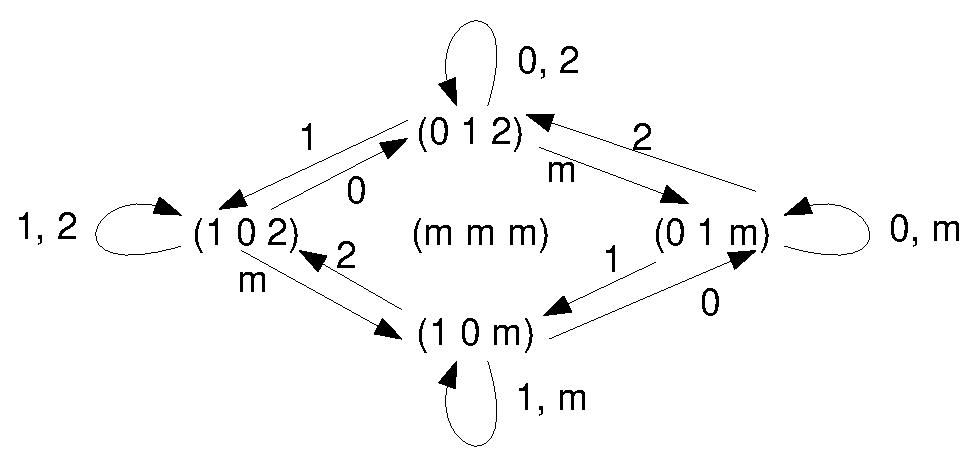
\includegraphics[width=0.7\textwidth]{2.theor/badpolicy}\\
  \caption{Граф для модельной стратегии вытеснения}\label{badpolicy}
\end{figure}

Для определения существования пути невытеснения может применяться
следующий алгоритм: сначала перебираются порядки на множестве чисел
$\{0, 1, ..., w-1\}$; обозначим очередной порядок как $i_1, i_2,
..., i_w$; строим множество вершин графа $V_1$, достижимых из $(0 1
... w-1)$ только по дугам с пометками $m$; если обнаружился цикл,
алгоритм завершается с ответом <<путь вытеснения есть>>; иначе
строим множество вершин $V'_1$, достижимых из $V_1$ по дугам с
пометкой $i_1$; строим множество вершин графа $V_2$, достижимых из
вершин $V'_1$ по дугам с пометками $m$; если обнаружился цикл,
алгоритм завершается с ответом <<путь вытеснения есть>>; иначе
строим множество вершин $V'_2$, достижимых из $V_2$ по дугам с
пометкой $i_2$; и так далее. Если цикл нигде не встретился и все
возможные порядки просмотрены, алгоритм завершается с ответом <<пути
вытеснения нет>>.

Граф для стратегий вытеснения \LRU и \PseudoLRU в случае
двух~-~ассоциативного буфера (для сокращения пометки заменены
штриховкой: дуга с пометка $m$ обозначена сплошной линией, дуга с
пометкой $0$ обозначена линией из точек, дуга с пометкой $1$
обозначена линией из пунктиров) изображен на
рисунке~\ref{lrupolicy}. В этом графе есть всего один цикл,
состоящий из сплошных дуг -- петля на вершине ($m$ $m$). Он включает
в себя вершину ($m$ $m$), поэтому в этом графе нет пути вытеснения.
В случае буферов с большим количеством секций ситуация будет
аналогичной.

Аналогичная ситуация будет и со стратегией вытеснения \FIFO (граф
для двух~-~ассоциативного буфера изображен на
рисунке~\ref{fifopolicy}). В этом графе тоже всего один цикл,
состоящий из сплошных дуг -- петля на вершине ($m$ $m$). Поскольку
этот цикл включает в себя вершину ($m$ $m$), то в этом графе нет
пути вытеснения. В случае буферов с большим количеством секций
ситуация будет аналогичной.

\begin{figure}[h]
\parbox{0.5\textwidth}{ \centering
  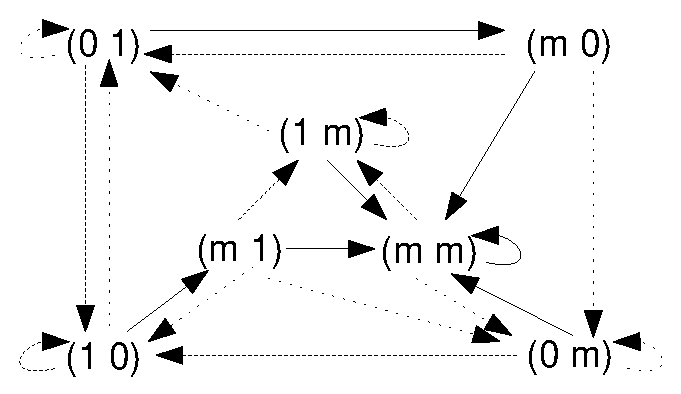
\includegraphics[width=0.45\textwidth]{2.theor/lrupolicy}
  \caption{Граф для стратегий вытеснения \LRU и \PseudoLRU с ассоциативностью 2}
  \label{lrupolicy}
} \vline
\parbox{0.5\textwidth}{ \centering
  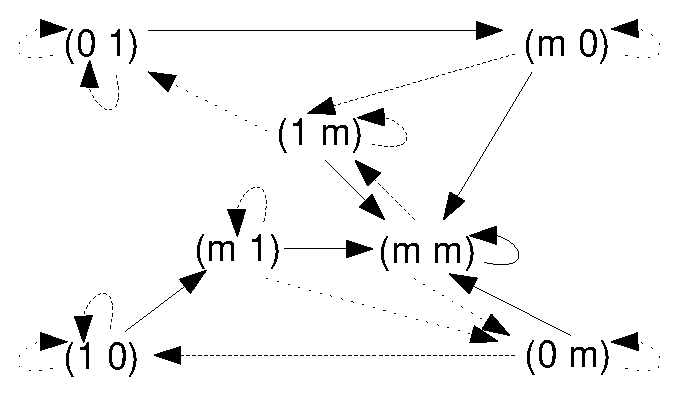
\includegraphics[width=0.45\textwidth]{2.theor/fifopolicy}
  \caption{Граф для стратегии вытеснения \FIFO с ассоциативностью 2}
  \label{fifopolicy}
}
\end{figure}


Таким образом, справедливо

\begin{utv} Зеркальный метод генерации
ограничений является полным для стратегий вытеснения \LRU, \FIFO и
\PseudoLRU.
\end{utv}
Это утверждение является важным, поскольку именно эти стратегии
вытеснения наиболее часто используются в микропроцессорах.

Доказательство теоремы~\ref{mirror_fullness} дает способ построения
последовательности инициализирующих тегов. Однако для некоторых
стратегий вытеснения такая последовательность будет избыточна и
существуют способы построения более коротких последовательностей
инициализирующих тегов. Следующая теорема дает линейное ограничение
для длины последовательности инициализирующих тегов от длины
тестового шаблона для стратегии вытеснения \LRU.

\begin{theorem}[Верхняя оценка для длины инициализирующей
последовательности тегов для стратегии вытеснения
\LRU]\label{thm_mirror_lenth_lru} \UpperBoundLRUMirror
\end{theorem}
Доказательство теоремы приведено в приложении~\ref{proofs}.
\begin{sld}
    Для длины последовательности инициализирующих тегов $m$ в случае
    стратегии вытеснения \LRU справедливо равенство:
      $$m = O(n)$$
\end{sld}

Следствие показывает, что зеркальный метод может быть эффективно
использован при стратегии вытеснения \LRU для поиска минимального
$m$ методом дихотомии.

\subsection{Совместно-зеркальная генерация}

Можно заметить, что при $m = 0$ формулировка ограничений для
зеркальной генерации становится частным случаем
теоремы~\ref{hit_miss_equations}. Это позволяет сформулировать
расширенный вариант этой теоремы, добавив туда <<зеркальную>>
инициализирующую последовательность тегов, и тем самым по сути этим
показывается соединение совместной и зеркальной генерации, ведь
даже, уменьшив множество констант $L_0$, система ограничений,
составленная на основе совместной генерации, может оказаться
несовместной -- в этом случае методом зеркальной генерации можно
будет добиться выполнения последовательности тестовых ситуаций,
указанных в тестовом шаблоне.

\begin{utv}\label{mirror_hit_miss_human} Пусть $L_0$ -- множество
адресов данных, расположенных в кэширующем буфере перед исполнением
первой инструкции тестового шаблона, $t_1, ..., t_m$ --
инициализирующая последовательность тегов. Тогда
\begin{itemize}
\item для инструкции с кэш-попаданием адреса $x$ следует добавить
следующую совокупность уравнений:
$$
\left[
   \begin{array}{l}
    x \in L_0 \wedge x~\mbox{все еще не вытеснен} \\
    x \in \{t_1, ..., t_m\} \wedge x~\mbox{не вытеснен} \\
    x~\mbox{внесен одним из кэш-промахов} \wedge \mbox{с тех пор не вытеснен} \\
   \end{array}
  \right.
$$

\item для инструкции с кэш-промахом адреса $x$ следует добавить следующую систему
уравнений ($\{x_i\}$ -- множество адресов данных в инструкциях с
кэш-промахами, расположенными до текущей инструкции):
$$
\left[
   \begin{array}{l}
    x \notin L_0 \wedge x \notin \{x_1, x_2, ..., x_n\} \\
    x \in \{t_1, ..., t_m\} \wedge x~\mbox{вытеснен и не внесен} \\
    x~\mbox{был вытеснен} \wedge \mbox{не был больше внесен в буфер}\\
  \end{array}
\right.
$$

\end{itemize}
\end{utv}

Некоторые решатели ограничений (\cite{Z3}) позволяют указывать веса
конъюнктов~-~ограничений в ДНФ. Эти веса могут использоваться для
построения решений, удовлетворяющих конъюнктам с минимальным или
максимальным суммарным весом. Таким образом, для дальнейшей
минимизации длины инициализирующей программы можно задавать
конъюнктам с $t_i$ больший вес, чем конъюнктам с $L_0$, и искать
решения с минимальным суммарным весом.

\subsection{Построение инициализирующей программы}

Если кэширующий буфер, для которого применяется зеркальный метод
генерации ограничений, подчинен некоторой таблице, то перед
инициализирующей последовательностью тегов ($t_1, t_2, ..., t_m$)
следует поместить инструкции, заполняющие нужные для этих тегов
строки таблицы. Например, перед последовательностью инициализирующих
обращений в TLB (допустим, что TLB является кэширующим буфером,
подчиненным таблице страниц виртуальной памяти) в таблицу страниц
надо поместить (если их там не было) страницы, соответствующие
инициализирующей последовательности тегов.

Если зеркальная генерация применяется к последовательностям тестовых
ситуаций для нескольких кэширующих буферов, то для каждого буфера
будет своя инициализирующая последовательность тегов. Может
ставиться задача построения более компактной инициализирующей
последовательности, объединяя некоторые обращения к буферам. Однако
эта задача не рассматривалась в работе.

\section{Единый взгляд на все предлагаемые методы}

\begin{figure}[p]
  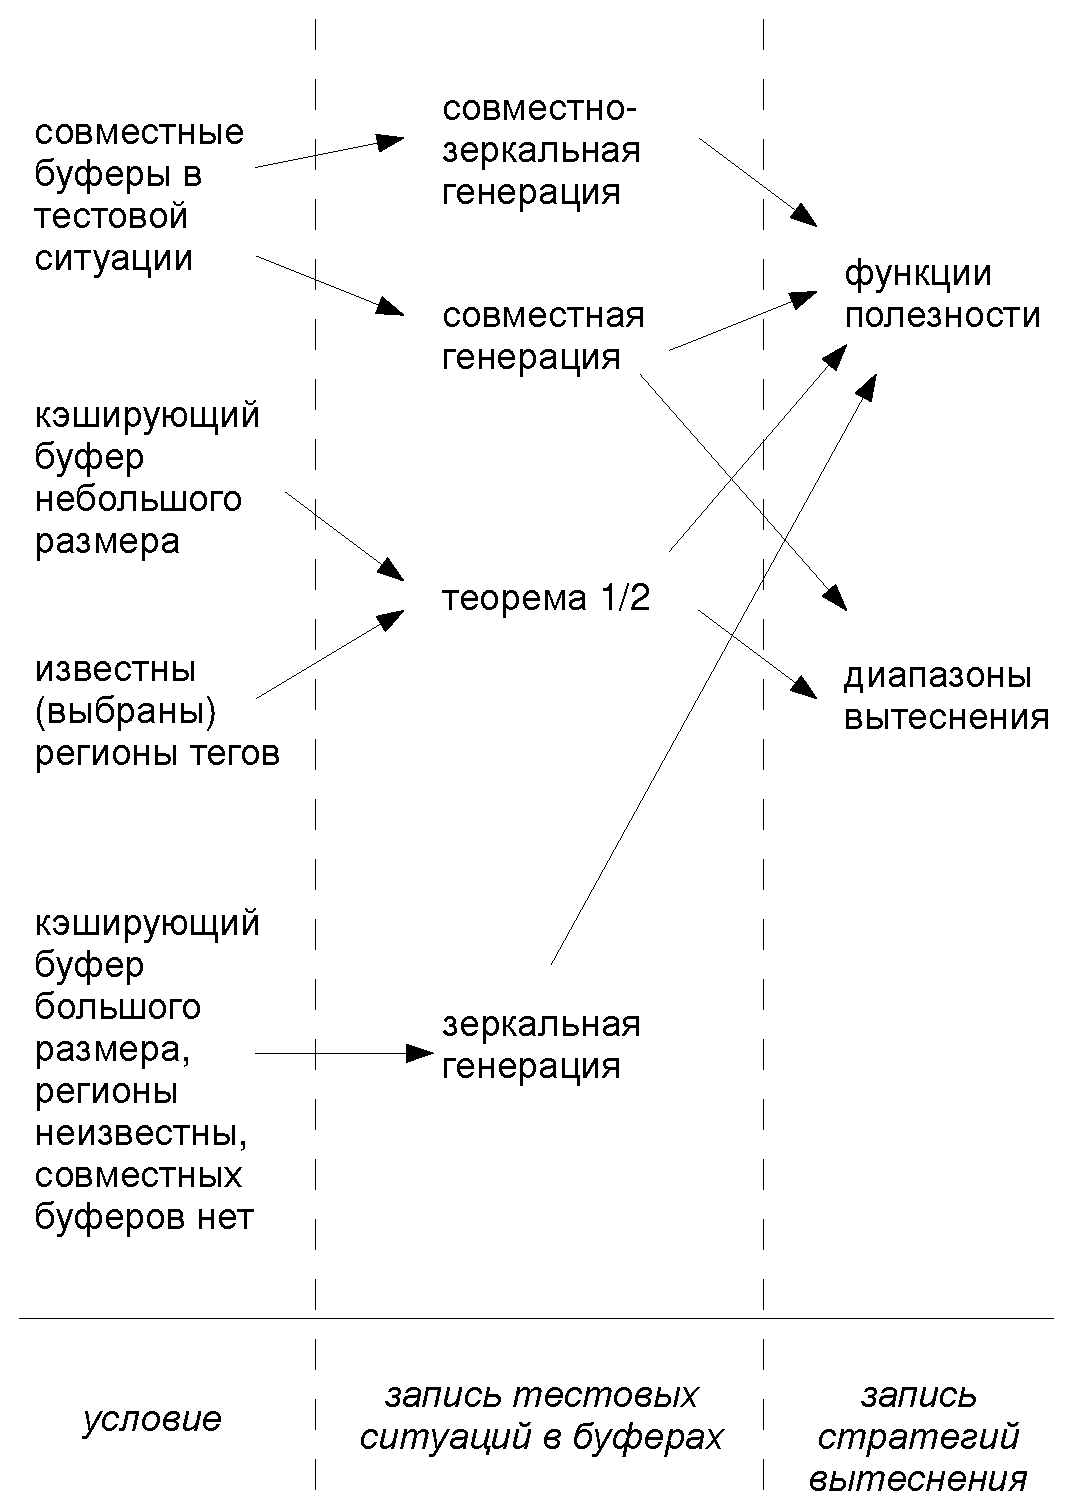
\includegraphics[width=0.9\textwidth]{2.theor/methods}\\
  \caption{Построение ограничений для тестовых шаблонов}\label{methods}
\end{figure}

На рисунке~\ref{methods} дан общий взгляд на предлагаемые методы
генерации ограничений для тестовых шаблонов. Надо записать в виде
ограничений последовательности кэш-попаданий и кэш-промахов (это
центральный столбец рисунка) -- это можно сделать с использованием
совместной генерации, зеркальной генерации, совместно-зеркальной
генерации или просто воспользовавшись
теоремой~\ref{hit_miss_equations}, в зависимости от свойств
тестового шаблона и MMU. Эти методы записи тестовых ситуаций в
кэширующих буферах позволяют использовать различные методы записи
стратегий вытеснения в виде ограничений (правый столбец рисунка).
Самих по себе методов записи тестовых ситуаций еще недостаточно для
генерации ограничений, поскольку они содержат в себе параметрическую
часть -- запись стратегии вытеснения. Для записи стратегий
вытеснения можно воспользоваться диапазонами вытеснения или
функциями полезности, к рассмотрению которых мы и переходим. Выбор в
пользу того или иного метода записи стратегии вытеснения
производится на основе возможностей решателя ограничений и
требований к эффективности желаемого генератора тестовых программ.

\begin{figure}[ht]
  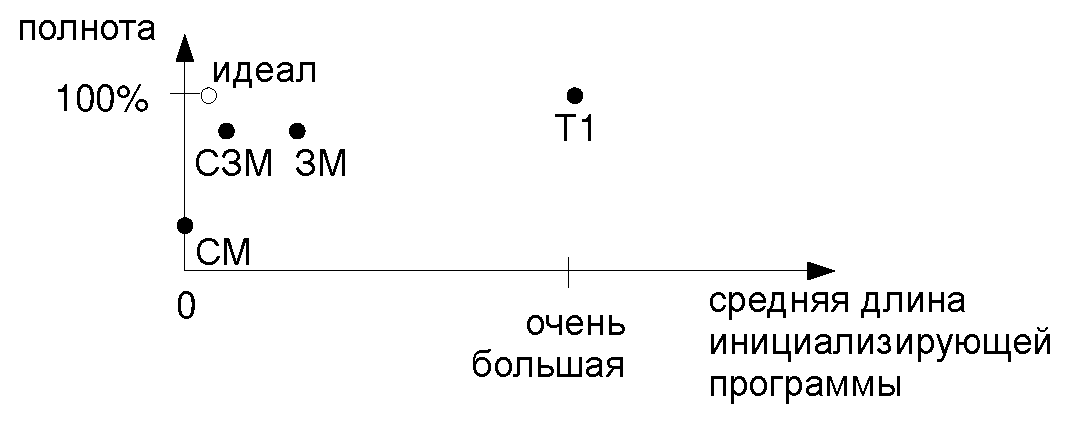
\includegraphics[width=0.8\textwidth]{2.theor/lenful}\\
  \caption{Сравнение полноты и средней длины инициализирующей программы,
  которую дают предлагаемые методы}\label{lenful}
\end{figure}

Рисунок~\ref{lenful} показывает сравнение средней длины
инициализирующих программ (без учета инструкций, не меняющих
кэширующие буферы и таблицы) и полноту предлагаемых методов.
Совместный метод генерации ограничений (СМ) не дает вообще никакой
инициализирующей программы, зато и применим он далеко не ко всем
тестовым шаблонам (в том числе и к тем, для которых возможно
построение тестовой программы) -- поэтому этот метод не является
полным. Совместно-зеркальный метод (СЗМ) и зеркальный метод (ЗМ)
дают неплохие показатели полноты, поскольку применимость этих
методов не так сильно зависит от тестового шаблона. Применение
теоремы~\ref{hit_miss_equations} (T1) без учета существующего
начального состояния микропроцессора (в противном случае эта теорема
уже не будет давать полного метода из-за большого размера
генерируемых ею ограничений -- $L_0$ должен быть выписан полностью)
дает полный метод всегда: если возможна хотя бы какая-нибудь
инициализация микропроцессора, она будет найдена. Однако ценою этого
является очень большая длина инициализирующей программы, поскольку
необходимо переинициализировать полностью весь микропроцессор, даже
если делать это не всегда обязательно.

%%%%%%%%%%%%%%%%%%%%%%%%%%%%%%%%%%%%%%%%%%%%%%%%%%%%%%%%%%%%%%%%%%%%%

\chapter{Методы генерации ограничений для описания стратегий вытеснения}

\section{Исследование стратегии вытеснения \PseudoLRU}

Стратегия вытеснения \LRU хоть и хорошо приближает поведение
кэширующего буфера к идеальному случаю (когда данные находятся в
буфере в тот момент, когда они нужны), однако все известные на
сегодняшний момент реализации для микропроцессоров требуют большого
количества дополнительной логики. Поэтому производятся поиски
стратегии вытеснения, близкой по эффективности к \LRU, но имеющей
реализацию с меньшими накладными расходами. Эти поиски привели к
стратегии вытеснения \PseudoLRU. Она определяется только для
кэширующих буферов с ассоциативностью, являющейся степенью двойки.
Стратегия вытеснения \PseudoLRU используется во многих
микропроцессорах архитектур PowerPC и
Pentium~\cite{FundamentalOfComputerOrganizationAndDesign}.

\subsubsection{Каноническое определение \PseudoLRU на бинарном дереве}

Следующее описание часто появляется в
литературе~\cite{FundamentalOfComputerOrganizationAndDesign} для
определения стратегии вытеснения \PseudoLRU. Оно формулируется на
упорядоченном бинарном дереве высоты $\log_2 w$, в листьях которого
подряд расположены теги набора (их количество равно $w$).
Вытесняющий тег помещается в дереве на место вытесняемого. Дуга,
идущая влево, помечена цифрой 0, дуга, идущая вправо, помечена
цифрой 1.

При кэш-попадании по некоторому тегу меняются пометки в нелистовых
вершинах пути от корня до соответствующей тегу листовой вершины (см.
рис.~\ref{pseudo_lru_hit}). А именно вершина получает метку
исходящей из нее дуги в пути до соответствующей тегу листовой
вершины. Т.е. если дуга, соответствующая пути, выходит влево,
вершина помечается цифрой 0, если вправо -- 1. Пометки на остальных
вершинах дерева не меняются.

\begin{figure}[h] \center
  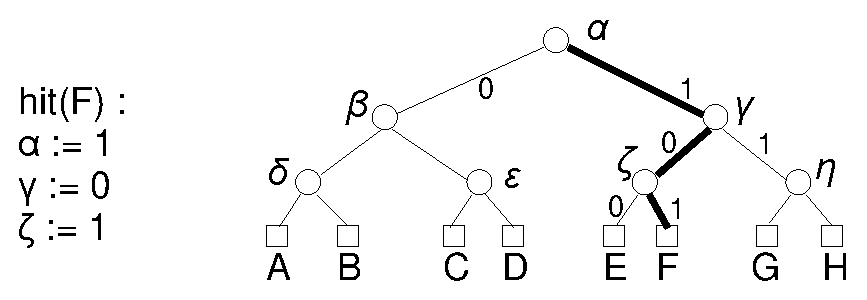
\includegraphics[width=0.7\textwidth]{2.theor/plruhit}\\
  \caption{Кэш-попадание для стратегия вытеснения \PseudoLRU
  (16-ассоциативный кэширующий буфер)}\label{pseudo_lru_hit}
\end{figure}

Поиск вытесняемого элемента производится следующим образом: на
основе пометок нелистовых вершин дерева определяется единственный
путь следующим образом: в каждой вершине пути выбирается
направление, противоположное пометке вершины. Если вершина помечена
цифрой 0, значит дуга пути к вытесняемому тегу идет из этой вершины
вправо. Если вершина помечена цифрой 1 -- влево. На место
вытесняемого элемента помещается вытесняющий, битовая строка
меняется так, будто к вытесняющему элементу было обращение с
кэш-попаданием. Пример того, как определяется вытесняемый элемент,
показан на рис.~\ref{pseudo_lru_miss}. Цветом нелистовых вершин
показаны их пометки: черным вершинам соответствует пометка 1, белым
-- 0. В изображенном на рисунке дереве в качестве вытесняемого тега
будет выбран тег D, к которому ведет путь
$\alpha-\beta-\varepsilon$.

\begin{figure}[h] \center
  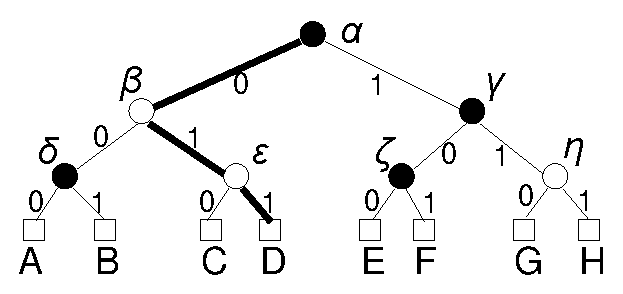
\includegraphics[width=0.5\textwidth]{2.theor/plrumiss}\\
  \caption{Определение вытесняемого элемента для стратегия вытеснения
  \PseudoLRU (16-ассоциативный кэширующий буфер)}\label{pseudo_lru_miss}
\end{figure}


\subsubsection{Каноническое определение \PseudoLRU на битовой строке}

Для каждого набора хранится битовая строка длины $w-1$, где $w$ --
ассоциативность кэширующего буфера. Каждая инструкция, обращающаяся
к набору, меняет эту битовую строку. Определение вытесняемого
элемента производится на основании только лишь этой битовой строки.

Во многих книгах приводятся следующее определение стратегии
вытеснения \PseudoLRU для случая
$w=4$~\cite{FundamentalOfComputerOrganizationAndDesign} (в этом
случае для каждого набора выделяется 3 бита $B_1$, $B_2$ и $B_3$):
$$ \left[
  \begin{array}{c|ccc}
          & B_1 & B_2 & B_3 \\ \hline
    \pi_0 & 0 & 0 & \textsf{X} \\
    \pi_1 & 0 & 1 & \textsf{X} \\
    \pi_2 & 1 & \textsf{X} & 0 \\
    \pi_3 & 1 & \textsf{X} & 1 \\
  \end{array}
\right]
$$

При кэш-попадании тега, расположенного в секции с номером $i$,
действует $i$'я строка матрицы (она помечена символом $\pi_i$).
Биты, напротив которых в $i$'й строке находится \textsf{X}, не
меняются. Биты, напротив которых в $i$'й строке находится число,
принимают значение, равное этому числу.

При кэш-промахе надо определить номер секции, в которой будут
заменены данные. Для этого используется инвертированная форма той же
матрицы:
$$
\left[
  \begin{array}{ccc|c}
    B_1 & B_2 & B_3 & \\ \hline
    1 & 1 & \textsf{X} & \rightarrow \pi_0 \\
    1 & 0 & \textsf{X} & \rightarrow \pi_1 \\
    0 & \textsf{X} & 1 & \rightarrow \pi_2 \\
    0 & \textsf{X} & 0 & \rightarrow \pi_3 \\
  \end{array}
\right]
$$

Выбирается строка, соответствующая текущему состоянию бит $B_1$,
$B_2$ и $B_3$: если напротив бита в строке находится число, бит
должен быть равен этому числу -- если напротив бита в строке
находится \textsf{X}, то требования на соответствующий бит нет.
Подходящая строка всегда будет существовать и она будет
единственной.

Изменение битовой строки можно демонстрировать на бинарном дереве и
наоборот. Битовая строка составляется из пометок вершин дерева,
начиная с корня и далее по слоям от левых к правым вершинам (см.
рис.~\ref{plru_bittree}).

\begin{figure}[h] \center
  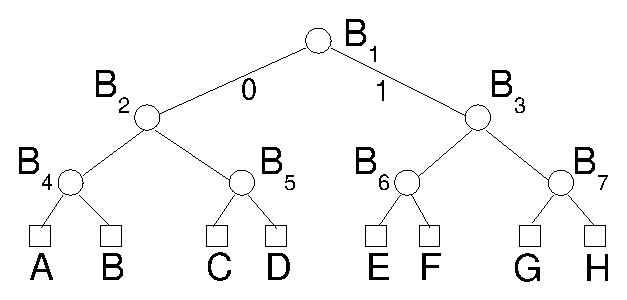
\includegraphics[width=0.5\textwidth]{1.review/plru}\\
  \caption{Битовая строка в бинарном дереве}\label{plru_bittree}
\end{figure}

Формализованное описание для всех допустимых $w$ в литературе не
приводится. Однако в дальнейшем для формулирования и доказательства
утверждений про стратегию вытеснения \PseudoLRU такое описание будет
необходимо. Для $w=8$ стратегия будет задаваться следующей матрицей:
$$
\left[
  \begin{array}{c|ccccccc}
          & B_1 & B_2 & B_3 & B_4 & B_5 & B_6 & B_7 \\ \hline
    \pi_0 & 0 & 0 & \textsf{X} & 0 & \textsf{X} & \textsf{X} & \textsf{X} \\
    \pi_1 & 0 & 0 & \textsf{X} & 1 & \textsf{X} & \textsf{X} & \textsf{X} \\
    \pi_2 & 0 & 1 & \textsf{X} & \textsf{X} & 0 & \textsf{X} & \textsf{X} \\
    \pi_3 & 0 & 1 & \textsf{X} & \textsf{X} & 1 & \textsf{X} & \textsf{X} \\
    \pi_4 & 1 & \textsf{X} & 0 & \textsf{X} & \textsf{X} & 0 & \textsf{X} \\
    \pi_5 & 1 & \textsf{X} & 0 & \textsf{X} & \textsf{X} & 1 & \textsf{X} \\
    \pi_6 & 1 & \textsf{X} & 1 & \textsf{X} & \textsf{X} & \textsf{X} & 0 \\
    \pi_7 & 1 & \textsf{X} & 1 & \textsf{X} & \textsf{X} & \textsf{X} & 1 \\
  \end{array}
\right]
$$

Следующее утверждение~\ref{wMinus1PseudoLRU} дает алгоритм
преобразования списка бит\\ $B_1, B_2, ..., B_{w{-}1}$ в результате
кэш-попадания и кэш-промаха. В его формулировке применяется двоичное
разложение. Биты разложения обозначаются последовательностью от
старших бит к младшим (т.е. список ($x_1~x_2~\dots~x_n$) обозначает
число $x_n + 2x_{n-1} + 4x_{n-2} + \dots + 2^n x_1$, $x_i \in \{0,
1\}$ для $i = 1, 2, \dots, n$). Например, 1 = (0 0 1), 6 = (1 1 0).

Везде далее символ $W$ будет обозначать $\log_2 w$. По определению
стратегии вытеснения \PseudoLRU $W$ будет натуральным числом.

\begin{utv}[$(w{-}1)$-представление стратегии вытеснения
\PseudoLRU]\label{wMinus1PseudoLRU}При кэш-попадании тега с позицией
$i = (i_1~i_2~\dots~i_W)$ происходит следующее изменение бит $B_1,
B_2, ..., B_{w{-}1}$:

\parbox{0.3\textwidth}{
  $$ \begin{array}{l}
  B_{k_1} := i_1 \\
  B_{k_2} := i_2 \\
  B_{k_3} := i_3 \\
  ...\\
  B_{k_W} := i_W \\
  \end{array}$$
} \vline
\parbox{0.7\textwidth}{
  $$ \begin{array}{l}
  k_1 = (1) \\
  k_2 = (1~i_1) \\
  k_3 = (1~i_1~i_2) \\
  ...\\
  k_W = (1~i_1~i_2~\dots~i_{W{-}1}) \\
  \end{array} $$
}
\\[1cm]

При кэш-промахе тега позиция $i = (i_1~i_2~\dots~i_W)$ определяется
следующим образом:

\parbox{0.3\textwidth}{
  $$ \begin{array}{l}
  i_1 = \neg B_{k_1} \\
  i_2 = \neg B_{k_2} \\
  i_3 = \neg B_{k_3} \\
  ...\\
  i_W = \neg B_{k_W} \\
  \end{array}$$
} \vline
\parbox{0.7\textwidth}{
  $$ \begin{array}{l}
  k_1 = (1) \\
  k_2 = (1~\neg B_{k_1}) \\
  k_3 = (1~\neg B_{k_1}~\neg B_{k_2}) \\
  ...\\
  k_W = (1~\neg B_{k_1}~\neg B_{k_2}\dots\neg B_{k_{W{-}1}}) \\
  \end{array} $$
}
\\[0.5cm]

Кроме того при кэш-промахе после определения позиции $i$ делается
преобразование бит $B_1, B_2, ..., B_{w{-}1}$ так, как в случае
кэш-попадания на $\pi_i$.
\end{utv}

\subsubsection{Определение \PseudoLRU на ветвях бинарного
дерева}\label{PseudoLRUonBranches}

Здесь будет показано, как из канонического определения \PseudoLRU
получить формулировку \PseudoLRU с точки зрения одного элемента
набора (каноническое определение рассматривает весь набор целиком и
для него формулирует правила работы с последовательностью бит $B_1,
B_2, ..., B_{w{-}1}$). Это определение ранее не встречалось в
литературе.

Сначала этот переход покажем на примере $w=4$. Первый шаг --- это
смена <<состояния>>: вместо последовательности бит $B_1, B_2, ...,
B_{w-1}$ будем рассматривать последовательность векторов бит
$\beta_0, \beta_1, \dots, \beta_{w-1}$ размера $W$. Каждый $\beta_i$
соответствует $i$'й листовой вершине бинарного дерева. Кэш-попадание
меняет теперь не внутренние вершины дерева, а листовые вершины.
Каждый $\beta_i$ будет представляться списком длины $W$ -- путь от
корня дерева к $i$'й листовой вершине: $\beta_0$ соответствует
($B_1$ $B_2$), $\beta_1$ соответствует ($B_1$ $\neg B_2$), $\beta_2$
соответствует ($\neg B_1$ $B_3$) и $\beta_3$ соответствует ($\neg
B_1$ $ \neg
B_3$).\\[0.5cm]

\parbox{0.2\textwidth}{ \centering
  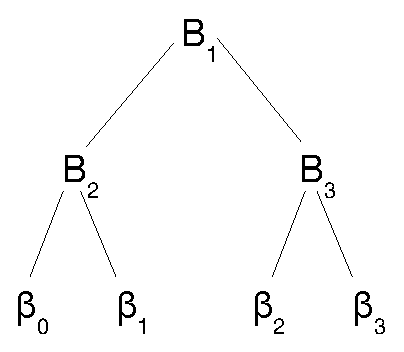
\includegraphics[width=0.2\textwidth]{1.review/btree}
}
\parbox{0.25\textwidth}{
$$ \left[
  \begin{array}{c|ccc}
          & B_1 & B_2 & B_3 \\ \hline
    \pi_0 & 0 & 0 & \textsf{X} \\
    \pi_1 & 0 & 1 & \textsf{X} \\
    \pi_2 & 1 & \textsf{X} & 0 \\
    \pi_3 & 1 & \textsf{X} & 1 \\
  \end{array}
\right]
$$
} $\stackrel{1}{\longrightarrow}$ %\vline
\parbox{0.4\textwidth}{
$$ \left[
  \begin{array}{c|cccc}
          & \beta_0 & \beta_1 & \beta_2 & \beta_3 \\ \hline
    \pi_0 & (0~0) & (0~1) & (1~\textsf{X}) & (1~\textsf{X}) \\
    \pi_1 & (0~1) & (0~0) & (1~\textsf{X}) & (1~\textsf{X}) \\
    \pi_2 & (1~\textsf{X}) & (1~\textsf{X}) & (0~0) & (0~1) \\
    \pi_3 & (1~\textsf{X}) & (1~\textsf{X}) & (0~1) & (0~0) \\
  \end{array}
\right]
$$
}

Заметим, что получилась симметричная матрица. На пересечении $\pi_i$
и $\beta_j$ располагается вектор, задающий изменение вектора в $j$'й
листовой вершине дерева при кэш-попадании $i$'й листовой вершины
дерева. Назовем позицию $i \oplus j$ \emph{относительной позицией}
$i$ относительно $j$. Рассмотрим отдельно каждый столбец
получившейся матрицы и переставим элементы столбца в порядке
увеличения относительных позиций.

\parbox{0.2\textwidth}{
$$ \left[
  \begin{array}{c|c}
          & \beta_0 \\ \hline
    \pi_0 & (0~0) \\
    \pi_1 & (0~1) \\
    \pi_2 & (1~\textsf{X}) \\
    \pi_3 & (1~\textsf{X}) \\
  \end{array}
\right]
$$
}\parbox{0.2\textwidth}{
$$ \left[
  \begin{array}{c|c}
          & \beta_1 \\ \hline
    \pi_0 & (0~1) \\
    \pi_1 & (0~0) \\
    \pi_2 & (1~\textsf{X}) \\
    \pi_3 & (1~\textsf{X}) \\
  \end{array}
\right]
$$
}\parbox{0.2\textwidth}{
$$ \left[
  \begin{array}{c|c}
          & \beta_2 \\ \hline
    \pi_0 & (1~\textsf{X}) \\
    \pi_1 & (1~\textsf{X}) \\
    \pi_2 & (0~0) \\
    \pi_3 & (0~1) \\
  \end{array}
\right]
$$
}\parbox{0.2\textwidth}{
$$ \left[
  \begin{array}{c|c}
          & \beta_3 \\ \hline
    \pi_0 & (1~\textsf{X}) \\
    \pi_1 & (1~\textsf{X}) \\
    \pi_2 & (0~1) \\
    \pi_3 & (0~0) \\
  \end{array}
\right]
$$
} $\stackrel{2}{\stackrel{\longrightarrow}{\pi^i_j \equiv \pi_{i
\oplus j}}}$

\parbox{0.24\textwidth}{
$$ \left[
  \begin{array}{c|c}
          & \beta_0 \\ \hline
    \pi^0_0 \equiv \pi_0 & (0~0) \\
    \pi^0_1 \equiv \pi_1 & (0~1) \\
    \pi^0_2 \equiv \pi_2 & (1~\textsf{X}) \\
    \pi^0_3 \equiv \pi_3 & (1~\textsf{X}) \\
  \end{array}
\right]
$$
}\parbox{0.24\textwidth}{
$$ \left[
  \begin{array}{c|c}
          & \beta_1 \\ \hline
    \pi^1_0 \equiv \pi_1 & (0~0) \\
    \pi^1_1 \equiv \pi_0 & (0~1) \\
    \pi^1_2 \equiv \pi_3 & (1~\textsf{X}) \\
    \pi^1_3 \equiv \pi_2 & (1~\textsf{X}) \\
  \end{array}
\right]
$$
}\parbox{0.24\textwidth}{
$$ \left[
  \begin{array}{c|c}
          & \beta_2 \\ \hline
    \pi^2_0 \equiv \pi_2 & (0~0) \\
    \pi^2_1 \equiv \pi_3 & (0~1) \\
    \pi^2_2 \equiv \pi_0 & (1~\textsf{X}) \\
    \pi^2_3 \equiv \pi_1 & (1~\textsf{X}) \\
  \end{array}
\right]
$$
}\parbox{0.24\textwidth}{
$$ \left[
  \begin{array}{c|c}
          & \beta_3 \\ \hline
    \pi^3_0 \equiv \pi_3 & (0~0) \\
    \pi^3_1 \equiv \pi_2 & (0~1) \\
    \pi^3_2 \equiv \pi_1 & (1~\textsf{X}) \\
    \pi^3_3 \equiv \pi_0 & (1~\textsf{X}) \\
  \end{array}
\right]
$$
}

После перехода к относительным позициям ($\pi^i_j$ -- это позиция
$\pi_j$ относительно $\pi_i$) все столбцы получились одинаковыми.
Иными словами, алгоритм изменения набора согласно стратегии
вытеснения \PseudoLRU на относительных позициях инвариантен
относительно абсолютной позиции вытесняемого тега. Тег вытесняется в
том случае, когда его вектор равен (1 1). Следующая теорема
формально доказывает этот факт.

Будем называть \emph{\PseudoLRU-ветвью позиции $i$} вектор
$(B_{k_1}^{\sigma_1}~B_{k_2}^{\sigma_2}~\dots~B_{k_W}^{\sigma_W})$,
в котором $\sigma_j = \neg i_j$, $k_j = (1~i_1~i_2~\dots~i_{j-1})$,
$j = 1, 2, \dots, W$, $i = (i_1~i_2~\dots~i_W)$ (двоичное
разложение). Степени определены стандартным образом: $B^1 \equiv B,
B^0 \equiv \neg B$.

\begin{theorem}[Инвариантность преобразования \PseudoLRU-ветвей относительными
позициями]\label{thm_pseudoLRU_invariant} \PseudoLRUInvariant
\end{theorem}
Доказательство теоремы приведено в приложении~\ref{proofs}.

Доказанный факт позволяет сформулировать определение стратегии
вытеснения \PseudoLRU, сфокусированное не на изменении всего набора,
а на изменении свойства одного тега набора. На этом определении
будут базироваться применения предлагаемых методов генерации
ограничений для стратегии вытеснения \PseudoLRU.

\begin{utv}[формулировка \PseudoLRU на ветвях бинарного дерева]
Сопоставим тегу вектор длины $W$. Каждая инструкция с этим тегом
делает этот вектор равным (0 0 ... 0). Тег является вытесняемым в
том и только в том случае, если этот вектор равен (1 1 ... 1).
Влияние других инструкций определяется относительной позицией их
тега относительно позиции данного тега. Если относительная позиция
принадлежит множеству $[\frac{w}{2^k},~\frac{w}{2^{k-1}}), k =
1,2,...,W$, то первые $k{-}1$ элементов вектора становятся равными
0, $k$'й элемент вектора становится равным 1, остальные элементы
вектора не меняются.
\end{utv}

Вектор длины $W$ будет соответствовать пути из корня бинарного
дерева в листовую вершину дерева, соответствующую данному тегу.
Будем называть процесс изменения элемента вектора
\emph{перекрашиванием вершины ветви}. Элементы вектора, равные 0,
будем называть \emph{белыми}, элементы вектора, равные 1, будем
называть \emph{черными}.

Говоря в терминах бинарного дерева, нелистовая вершина в ветви к
данной листовой вершине будет <<белой>>, если дуга от нее идет
налево и она помечена цифрой 1 или дуга от нее идет направо и она
помечена цифрой 0 (т.е. в том случае, когда направление дуги из нее
соответствует пометке этой дуги). Нелистовая вершина будет
называться <<черной>>, если направление дуги из нее не соответствует
пометке этой дуги. Вытесняется тот тег набора, путь к которому
полностью состоит из несоответствующих дуг. На рисунке~\ref{recolor}
изображен процесс перекрашивания ветви, ведущей в А, под действием
кэш-попадания в C (для сокращения показана только ветвь в А без
остальной части дерева). Так как путь из корня в C совпадает из
верхних двух вершин, то они перекрашиваются в белый цвет. Дуга из
третьей вершины пути в С не совпадает с дугой пути в А, поэтому
третья вершина перекрашивается в черный цвет. Остальные вершины
ветви остаются без изменений.

\begin{figure}[h] \center
  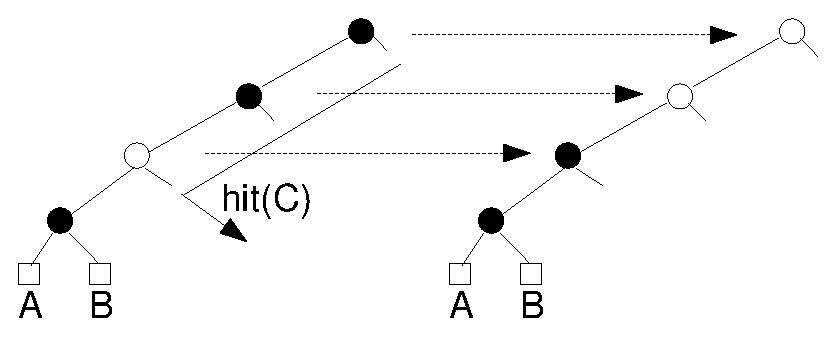
\includegraphics[width=0.8\textwidth]{1.review/recolor}\\
  \caption{Перекрашивание ветви в А}\label{recolor}
\end{figure}


Определение стратегии вытеснения \PseudoLRU на ветвях дерева
является связующим звеном между каноническим определением (например,
на битовой строке) и определением с помощью таблицы вытеснения,
поскольку ветвь -- это и есть позиция, которая меняется точно так
же, как и позиция в перестановке согласно таблице вытеснения.


\section{Метод перебора диапазонов вытеснения записи стратегии
вытеснения в виде ограничений}

В разделе рассматривается метод составления ограничений, описывающих
стратегию вытеснения. Метод применяется к стратегиям вытеснения, для
которых можно определить \emph{метрику вытеснения} и \emph{диапазон
вытеснения}. Составляемые ограничения представляют собой дизъюнкции
по всем возможным диапазонам вытеснения для данного вытесняемого
тега. В разделе приведены метрики вытеснения и ограничения для трех
наиболее часто использующихся в микропроцессорах стратегий
вытеснения --- \LRU, \FIFO и \PseudoLRU.

Неформально говоря, \emph{диапазон вытеснения} -- это непрерывная
часть тестового шаблона, заканчивающаяся в данной инструкции (это
т.н. \emph{конец диапазона вытеснения}), которая непосредственно
влияет на вытеснение некоторого элемента кэширующего буфера.
Зачастую \emph{началом диапазона вытеснения} является инструкция, в
которой осуществляется последнее обращение к вытесняемому элементу.

\emph{Метрикой вытеснения} будем называть функцию от текущего
состояния кэширующего буфера и части тестового шаблона. Она
максимальна в конце диапазона вытеснения и минимальна в начале
диапазона вытеснения. Определение диапазона вытеснения будет
производиться на основе такой метрики.

\subsection{Метод перебора диапазонов вытеснения для стратегии
вытеснения \LRU}\label{LRU_constraints}

\LRU (Least Recently Used) --- это стратегия вытеснения,
определяющая вытесняемые данные как наименее используемые. Она
эффективна для алгоритмов, обладающих свойством локальности данных,
т.е. чаще использующих те данные, к которым недавно происходило
обращение. Эта стратегия используется, например, в микропроцессорах
архитектуры MIPS~\cite{mips64_II}.

Стратегия вытеснения \LRU обычно определяется с использованием
счетчиков обращений. Для каждого элемента кэширующего буфера
вводится счетчик обращений к нему. Каждое обращение увеличивает
счетчик. Вытесняемым будет элемент с минимальным счетчиком.
Поскольку границы значений счетчика неизвестны, формулирование
метрики вытеснения на основе счетчика провести сложно.

Другой способ описания \LRU основан на введении порядка на элементах
набора (т.е. набор представляется списком элементов). После каждой
инструкции элементы переупорядочиваются согласно следующим правилам
(см.рис.~\ref{lru1}):
\begin{itemize}
\item при кэш-попадании элемент, соответствующий адресу инструкции,
перемещается в начало, остальные элементы от первого до данного
сдвигаются на одну позицию;
\item при кэш-промахе вытесняется последний элемент, в начало
вставляется элемент, вызвавший промах.
\end{itemize}

\begin{figure}[h] \center
  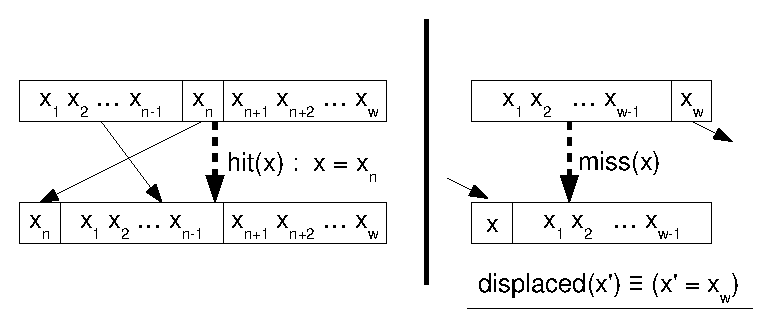
\includegraphics[width=0.6\textwidth]{2.theor/lru1}\\
  \caption{Стратегия вытеснения \LRU (w --- ассоциативность кэширующего буфера)
  --- реализация на списках}\label{lru1}
\end{figure}

Это описание подходит для определения метрики вытеснения: ею будет
\emph{индекс элемента в этом списке}. Эта метрика максимальна в
момент вытеснения (индекс равен длине списка). Минимальное значение
она принимает в момент кэш-попадания на этот элемент (т.к. он
переносится в самое начало, индекс становится равным 1). Значит,
применение перебора диапазонов вытеснения возможно (выделена метрика
вытеснения), началом диапазонов вытеснения будет последнее обращение
к вытесняемому элементу.

\begin{utv}[метрика вытеснения для стратегии вытеснения \LRU]
Метрикой вытеснения элемента для стратегии вытеснения \LRU является
индекс элемента в наборе согласно порядку последних обращений.
Диапазон вытеснения начинается в инструкции, последний раз
обращающейся к элементу (или в начальном состоянии, если инструкции
тестового шаблона к этому элементу не обращаются).
\end{utv}

Другое объяснение таким диапазонам вытеснения можно дать, исходя из
самого определения \LRU. А именно, если элемент должен стать \LRU,
т.е. наиболее неиспользуемым, все остальные элементы, наоборот,
должны быть хотя бы раз использованы (т.е. к ним должны быть
обращения до вытесняющей инструкции). Иными словами, чтобы элемент
был вытеснен, необходимо и достаточно, чтобы между последним
обращением к нему и вытеснением были обращения ко всем элементам
текущего состояния кэширующего буфера, кроме него (см.
рис.~\ref{lru-ranges}).

\begin{figure}[h] \center
  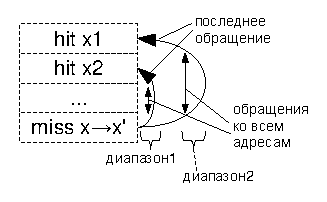
\includegraphics[width=0.4\textwidth]{2.theor/lru}\\
  \caption{Диапазоны вытеснения для стратегии вытеснения LRU}\label{lru-ranges}
\end{figure}

Запишем в виде уравнений на множества эту логику~\cite{my_syrcose_2009}. Предикат\\
$displaced(x')$ будет представлен дизъюнкцией уравнений --- каждый
элемент дизъюнкции соответствует некоторому диапазону вытеснения.
Тогда для диапазона вытеснения к инструкции, обращающейся к адресу
$y$ надо составить такую систему уравнений ($x_1, x_2, ..., x_n$ --
множество адресов, к которым происходят обращения внутри диапазона
вытеснения (как с кэш-попаданиями, так и с кэш-промахами, а также
элементы начального состояния, если диапазон начинается там), $L$ --
выражение для состояния кэширующего буфера перед инструкцией, в
которой вытесняется $x'$):
$$
\left\{
   \begin{array}{l}
    x' = y \\
    \{x_1, x_2, ..., x_n\} \cap R(y) = (L \setminus \{y\}) \cap R(y)\\
   \end{array}
  \right.
$$

Следующая теорема обосновывает и упрощает эту систему уравнений.
Функциональный символ $R$ используется в смысле множества адресов
того же региона.
\begin{theorem}[Уравнение для \LRU]\label{LRU_equation} \DiapazonLRU
\end{theorem}

Доказательство теоремы приведено в приложении~\ref{proofs}.

\subsection{Метод перебора диапазонов вытеснения для стратегии
вытеснения \FIFO}

\FIFO (First-In First-Out) -- это стратегия вытеснения, определяющая
вытесняемые данные согласно принципу очереди FIFO. Например, в
микропроцессоре PowerPC 970FX вытеснение из небольшого буфера,
хранящего последние преобразованные эффективные адреса в физические,
D-ERAT происходит согласно \FIFO~\cite{PowerPC970FXUserManual}.

Стратегия \FIFO может быть описана на основе порядка на элементах
набора (т.е. набор представляется списком элементов). После каждой
инструкции элементы переупорядочиваются согласно следующим правилам
(см.рис.~\ref{fifo1}):
\begin{itemize}
\item при кэш-попадании порядок элементов не меняется;
\item при кэш-промахе вытесняется последний элемент, в начало
вставляется элемент, вызвавший промах.
\end{itemize}

\begin{figure}[h] \center
  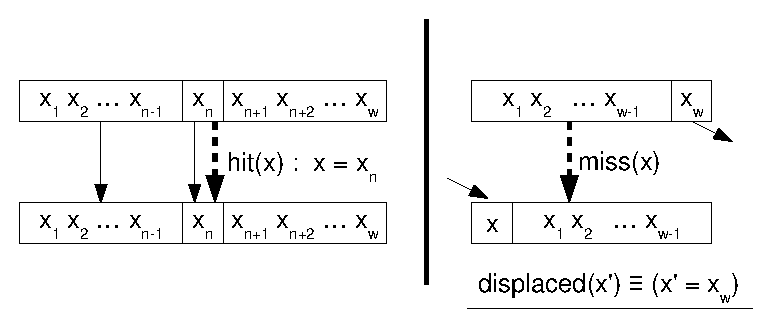
\includegraphics[width=0.6\textwidth]{2.theor/fifo1}\\
  \caption{Стратегия вытеснения \FIFO (w --- ассоциативность
  кэширующего буфера)}\label{fifo1}
\end{figure}

Отличие от \LRU лишь в том, что при \FIFO не происходит перестановки
элементов набора при возникновении кэш-попадания. Поэтому таблица
вытеснения~\cite{policy_tables} для стратегии вытеснения \FIFO будет
выглядеть так, как изображено на рисунке~\ref{fifo_policy_table}.

\begin{figure}
$$
  \left[
    \begin{array}{c|cccccc}
      \pi_0 & 0 & 1 & 2 & 3 & \dots & w-1 \\
      \pi_1 & 0 & 1 & 2 & 3 & \dots & w-1 \\
      \pi_2 & 0 & 1 & 2 & 3 & \dots & w-1 \\
      \vdots &  &  &  & & & \\
      \pi_{w-1} & 0 & 1 & 2 & 3 & \dots & w-1 \\
      \pi_m & m & 0 & 1 & 2 & \dots & w-2 \\
    \end{array}
  \right]
$$
\caption{Таблица вытеснения для \FIFO}\label{fifo_policy_table}
\end{figure}

Аналогично \LRU в качестве метрики вытеснения можно взять индекс
элемента в списке, что дает возможность использовать перебор
диапазонов вытеснения для описания стратегии вытеснения \FIFO.
Началом диапазона вытеснения будет внесение элемента в кэширующий
буфер, концом диапазона вытеснения -- его вытеснение. При
составлении ограничений все инструкции с кэш-попаданиями внутри
диапазона будем игнорировать (они не влияют на вытеснение с точки
зрения \FIFO). Тогда \emph{\FIFO будет выполнено в том случае, когда
в диапазоне встречаются все теги кэширующего буфера, хранящиеся в
нем перед вытеснением, без самого вытесняемого тега}.

\begin{utv}[метрика вытеснения для стратегии вытеснения \FIFO]
Метрикой вытеснения тега для стратегии вытеснения \FIFO является его
индекс в наборе согласно порядку последних обращений. Диапазон
вытеснения начинается в инструкции c кэш-промахом, последний раз
обращающейся к вытесняемому тегу (или в начальном состоянии, если
инструкции тестового шаблона к этому тегу не обращаются).
\end{utv}

Запишем в виде уравнений на множества эту логику~\cite{my_nivc_2009}. Предикат\\
$displaced(y')$ будет представлен дизъюнкцией уравнений -- каждый
элемент дизъюнкции соответствует некоторому диапазону вытеснения.
Тогда для диапазона вытеснения к инструкции, обращающейся к адресу
$y$, надо составить такую систему уравнений ($y_1, y_2, ..., y_n$ --
множество адресов, к которым происходят обращения внутри диапазона
вытеснения \textbf{с кэш-промахами}, а также элементы начального
состояния, если диапазон начинается там, $L$ -- выражение для
состояния кэширующего буфера для инструкции, вытесняющей $y'$):
\begin{theorem}[Уравнение для \FIFO]\label{FIFO_equation} \DiapazonFIFO
\end{theorem}

Функциональный символ $R$ используется в смысле множества адресов
того же региона. Доказательство теоремы приведено в приложении~\ref{proofs}.

\subsection{Метод перебора диапазонов вытеснения для стратегии
вытеснения \PseudoLRU}

Воспользуемся определением \PseudoLRU на ветвях бинарного дерева
(см. п.~\ref{PseudoLRUonBranches}). Согласно этому определению при
кэш-попадании (или внесении в кэширующий буфер) тега его ветвь
<<обнуляется>>, т.е. становится равной (0 0 ... 0). Каждая
последующая инструкция перекрашивает часть этой ветви до тех пор,
пока к некоторому кэш-промаху эта ветвь не станет равной (1 1 ...
1). В этом случае данный тег будет вытеснен. Таким образом, в
качестве метрики вытеснения предлагается использовать количество
единиц в ветви. Это количество максимально в момент вытеснения и
минимально в момент кэш-попадания (или внесения) данного тега.
Применение перебора диапазонов вытеснения для описания \PseudoLRU
возможно: началом диапазона будет последнее обращение к тегу
(листовой вершине дерева), концом диапазона будет вытесняющая этот
тег инструкция.

\begin{utv}[метрика вытеснения для стратегии вытеснения \PseudoLRU]
Метрикой вытеснения элемента для стратегии вытеснения \PseudoLRU
является количество вершин в ветви к вытесняемой листовой вершине с
пометками, противоположными пометкам при прохождении по ветви при
кэш-попадании. Диапазон вытеснения начинается в инструкции,
последний раз обращающейся к листовой вершине (или в начальном
состоянии, если инструкции тестового шаблона к этой листовой вершине
не обращаются).
\end{utv}

%Отличием этой метрики вытеснения от метрики вытеснения для \LRU или
%\FIFO является \emph{немонотонность}. Обращение к листовым вершинам,
%лежащим близко к данной, может перекрасить в белый цвет некоторые до
%этого бывшие черными вершины, что уменьшит метрику, но не сделает ее
%значение минимальной. Как будет продемонстрировано ниже, монотонные
%метрики вытеснения позволяют строить более компактные ограничения,
%чем немонотонные. Метрика вытеснения не является единственной для
%стратегии вытеснения, поэтому поиск монотонной метрики вытеснения
%является еще одним способом упрощения ограничений.

Осталось записать уравнения, описывающие предложенные диапазоны
вытеснения. Каждый тег кэширующего буфера снабдим \emph{позицией} --
номером этого элемента среди листовых вершин дерева. Будем
обозначать позицию буквой $\pi$. Предикат $displaced(x')$ будет
представлен дизъюнкцией уравнений -- каждый элемент дизъюнкции
соответствует некоторому диапазону вытеснения. Тогда для диапазона
вытеснения к инструкции, обращающейся к адресу $x_1$ c позицией
$\pi_1$ надо составить такую систему уравнений (~$x_2, x_3, ...,
x_n$ -- множество адресов, к которым происходят обращения внутри
диапазона вытеснения, $\pi_2, \pi_3, ..., \pi_n$ -- соответствующие
им позиции, $\delta_i = \pi_i \oplus \pi', i = 2,3,\dots,n$, --
относительные позиции ):

\begin{figure}[h] \center
  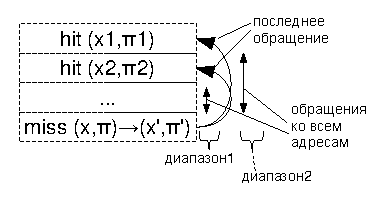
\includegraphics[width=0.5\textwidth]{2.theor/plru-ranges}\\
  \caption{Диапазоны вытеснения для стратегии вытеснения \PseudoLRU}
\end{figure}

$$
\left\{
\begin{array}{l}
x' = x_1\\
\pi' = \pi_1\\
\pi = \pi'\\
((0~op_x~\delta_2)~op_x~\delta_3) ... ~op_x~\delta_n  = w-1\\
\end{array}
\right.
$$

Операция $op_x$ выполняет очередной шаг по <<перекрашиванию>> ветви,
ведущей в элемент $x$. Она может быть определена следующей формулой:

$$X~op_x~\delta \equiv \mbox{~if~} R(X) \neq R(x) \mbox{~then~} X \mbox{~else~} (X \&
\delta_{<1>}) | \delta_{<0>} \mbox{~end~}$$

где \& -- побитовая конъюнкция, | -- побитовая дизъюнкция,
$\delta_{<1>} = 2 * \delta_{<0>} - 1$, а $\delta_{<0>} = 2^{[\log_2
\delta]}$ может быть определено следующим переборным способом:
$\delta_{<0>} = \mbox{~if~} 1 \leqslant \delta < 2 \mbox{~then~} 1
\mbox{~elsif~} 2 \leqslant \delta < 4 \mbox{~then~} 2 \mbox{~elsif~}
... \mbox{~else~} w \mbox{~end~}$. Другой способ получения
$\delta_{<0>}$ и $\delta_{<1>}$ удобно применять при побитовом
рассмотрении $\delta$: $\delta_{<0>} = (\delta_{<1>} + 1) \gg 1$,
$\delta_{<1>}[i] = \delta[1] \vee \delta[2] \vee ... \vee
\delta[i]$, где символом $d[i]$ обозначен $i$'й бит числа $d$, биты
нумеруются со старших к младшим.


%%%%%%%%%%%%%%%%%%%%%%%%%%%%%%%%%%%%%%%%%%%%%%%%%%%%%%%%%%%%%%%%%%%%

\pagebreak
\section{Метод функций полезности записи стратегии вытеснения в виде
ограничений}

В разделе рассматривается метод составления ограничений, описывающих
стратегию вытеснения, для которых можно определить метрик
вытеснения. Стратегия вытеснения описывается ограничением сверху на
количество \emph{полезных} инструкций (т.е. помогающих вытеснению).
В разделе приведены метрики полезности и ограничения для трех
наиболее часто использующихся в микропроцессорах стратегий
вытеснения -- \LRU, \FIFO и \PseudoLRU. Освещается понятие
\emph{монотонной метрики вытеснения}, которая является залогом более
компактной системы ограничений.

Пусть для стратегии вытеснения сформулирована метрика вытеснения (ее
значение максимально в вытесняющей инструкции). Будем называть
инструкцию \emph{полезной}, если она увеличивает метрику на этапе
монотонного увеличения метрики до максимального значения (см.
рис.~\ref{useful}).

\begin{figure}[h] \center
  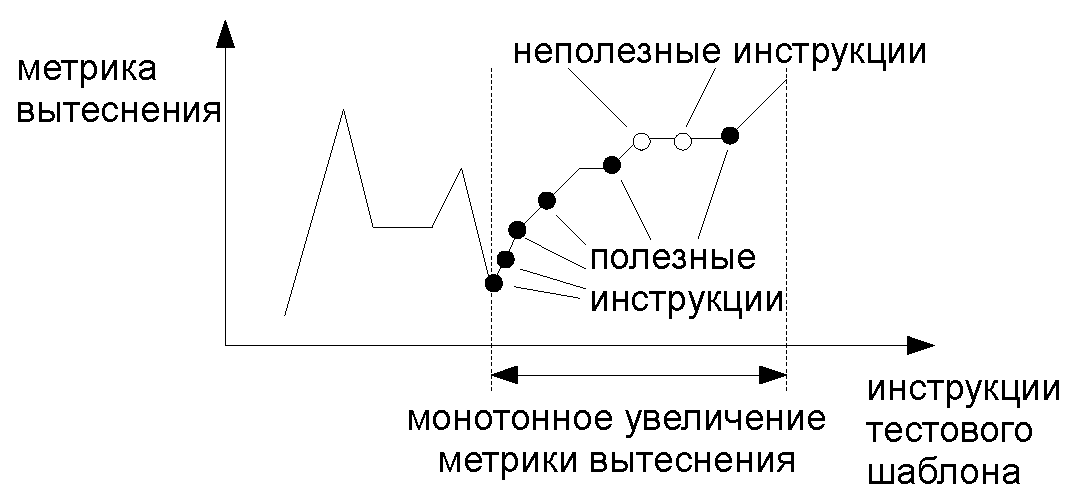
\includegraphics[width=0.6\textwidth]{2.theor/useful}\\
  \caption{К определению полезных инструкций}\label{useful}
\end{figure}

Тогда вытеснение будет происходить в том случае, когда количество
полезных инструкций превысит некоторое константное количество.
Вытеснение не будет происходить, если количество полезных инструкций
не превысит некоторой константной верхней границы. Количество
полезных инструкций можно записать в виде суммы
переменных-полезностей, каждая такая переменная соответствует своей
инструкции и равна 1 тогда и только тогда, когда инструкция является
полезной, и 0 тогда и только тогда, когда инструкция не является
полезной. Иными словами, ограничение будет иметь вид $\sum_{i=1}^n
u(x_i) < N$ или $\sum_{i=1}^n u(x_i) = N$, где $u(x_i)$ --
\emph{функция полезности} (равна 1, если $x_i$ -- полезная
инструкция, и равна 0, если $x_i$ не является полезной инструкцией).

Функции полезности не являются единственными. Например, для стратегии вытеснения \LRU можно привести такие две различные функции полезности (далее для одной из них будет показано, что она действительно является функцией полезности):
\begin{itemize}
  \item $u_x(x_i) \equiv (x \notin \{x_i, x_{i+1}, ..., x_n\} \wedge R(x_i) = R(x) \wedge x_i \notin \{x_{i+1}, x_{i+2}, ..., x_n\})$ -- инструкция считается полезной, если она расположена после последнего обращения к $x$, обращается в тот же регион, что и регион $x$, и является последним обращением к своему тегсету перед финальным обращением к $x$;
  \item $u_x(x_i) \equiv (x \notin \{x_i, x_{i+1}, ..., x_n\} \wedge R(x_i) = R(x) \wedge \\ \bigwedge_{j=1,2,...,i-1} (x \in \{x_j, x_{j+1}, ..., x_{i-1}\} \vee x_j \neq x_i))$ -- инструкция считается полезной, если она расположена после последнего обращения к $x$, обращается в тот же регион, что и регион $x$, и является первым обращением к своему тегсету после последнего обращения к $x$.
\end{itemize}

\subsection{Метод функций полезности для стратегии
вытеснения \LRU}

Функцией полезности является номер вытесняемого элемента согласно
порядку счетчика \LRU (см. рис.~\ref{lru1}). Значит, полезной будет
инструкция, переставляющая вытесняемый элемент в этом порядке к
концу. Такими инструкциями являются все кэш-промахи (поскольку они
вытесняют последний элемент с передвижением всех остальных на одну
позицию к концу, в том числе будет передвинут и данный вытесняемый
элемент) и кэш-попадания к элементам, находившимся ближе к концу,
чем данный вытесняемый (потому как при кэш-попадании они
передвинутся в самое начало, а все элементы от начала и до них
сдвинутся на одну позицию к концу, в том числе и данный
вытесняемый).

Осталось выразить эту идею в виде ограничений~\cite{my_ewdts_2009}.
Для этого удобно использовать формулировку тестовых ситуаций в
кэширующем буфере из утверждения~\ref{hit_miss_human}. Символом
$\lambda_\delta$ будет обозначаться элемент домена -- начального
состояния буфера -- с индексом $\delta$ по порядку \LRU, $1
\leqslant \delta \leqslant w$. Индекс 1 обозначает самый молодой
элемент, индекс $w$ обозначает самый старый элемент.

Применение полезностей эффективно в том случае, когда домен имеет
небольшой размер (такие домены как раз обеспечивает совместная
генерация ограничений). В этом случае можно перебрать все элементы
домена (это и будут $\lambda_\delta$) и составить для них свои
полезности, причем для каждого элемента будет известен индекс по
порядку \LRU ($\delta$). Ограничение, описывающее стратегию
вытеснения, будет при этом иметь вид дизъюнкции по элементам домена.

Если вытесняемый элемент был в начальном состоянии (пусть это
$\lambda_\delta$) и к нему не было обращений, то для его вытеснения
необходимо $w-\delta + 1$ полезных инструкций, потому что столько
раз надо подвинуть элемент с индексом $\delta$ в \LRU-списке в
сторону к концу (к элементам с индексом $w$), чтобы он вышел за
границу списка (иными словами, чтобы он был вытеснен).

Если вытесняемый элемент был в начальном состоянии и к нему было
обращение, то для его вытеснения необходимо $w$ инструкций, так как
во время обращения элемент был поставлен в самое начало \LRU-списка.
То же справедливо для внесенных в кэширующий буфер новых тегсетов --
чтобы их вытеснить, надо так же $w$ полезных инструкций, чтобы
переместить их к концу \LRU-списка.

В таблице~\ref{hit_miss_table} приведены все функции полезности для
кэш-попаданий и кэш-промахов. Доказательство корректности приведенных
 в ней формул (т.е. доказательство того, что эти формулы действительно
 описывают \LRU) важны, но не представляют самостоятельного результата.
Поэтому они были вынесены за пределы основной части диссертации и
находятся в приложении~\ref{proofs}.

Несколько слов об уменьшении ограничений для всех случаев.
Представленные ограничения достаточны для полного описания
кэш-попаданий и кэш-промахов. В некоторых случаях однако их
количество можно сократить, используя следующие эвристики:
\begin{itemize}
\item \emph{тождественные ограничения мощности}: ограничения вида\\
$\sum_{i=1}^n a_i \leqslant C$ можно не включать в конъюнкцию, если
$C > n$; если $C < 0$, то вся конъюнкция несовместна; если $C = 0$
или $C = n$, то ограничение мощности можно сразу расписать в
конъюнкцию вида $\bigwedge_i (a_i = \alpha)$, где $\alpha = 0$, если
$C = 0$, и $\alpha = 1$, если $C = n$; аналогично с ограничениями
вида $\sum_{i=1}^n a_i \geqslant C$;
\item \emph{ограничения на $\delta$}: если $\delta + 1 < w$, то
функция полезности, в которую входит множество
$\{\lambda_{\delta+1}, ..., \lambda_w\}$, равна 0;
\item \emph{пересечение тегсетов}: при построении ограничений для
нескольких кэширующих буферов, чьи тегсеты могут быть битовыми
полями (как, например, в случае кэш-памяти и буфера TLB в
микропроцессоре MIPS~\cite{mips64_III}), возникают конъюнкции
ограничений вида $x \in \{x_1, ..., x_n\}~\wedge\\\widehat{x} \notin
\{ \widehat{y_1}, ..., \widehat{y_m} \}$, где $x$ -- тег в одном
буфере, а $\widehat{x}$ -- тег в другом буфере; поскольку
неравенство битовых полей чисел влечет неравенство самих чисел, то
общие тегсеты среди $x_1, ..., x_n$ и $y_1, ..., y_m$ можно
исключить из ограничения на $x$.
\end{itemize}


\subsection{Метод функций полезности для стратегии
вытеснения \FIFO}

Из сравнения таблиц вытеснения для \FIFO и \LRU следует, что
стратегию вытеснения \FIFO можно воспринимать, как частный случай
\LRU, в котором кэш-попадание не меняет состояния списка \LRU.
Поэтому и ограничения с функциями полезности для \FIFO будем строить
на основе уже сформулированных и обоснованных ограничений с
функциями полезности для \LRU. Кроме того все инструкции с
кэш-попаданиями, поскольку они не влияют на вытеснение, можно вообще
исключить из ограничений. Получившиеся ограничения показаны в
таблице~\ref{fifo_table}. Доказательства корректности и полноты этих
ограничений идентичны доказательствами для \LRU. Символом
$[\sum\limits^n_{i=1}]_{miss} u(x_i)$ обозначена сумма $u(x_i)$, где
$i=1..n$ и тегсет $x_i$ дает в своей инструкции кэш-промах.


\subsection{Метод функций полезности для стратегии
вытеснения \PseudoLRU}

При использовании функций полезности не происходит выделение участка
тестового шаблона, непосредственно влияющего на вытеснение данного
тегсета. Считается, что это влияние начинается с момента появления
тегсета в кэширующем буфере. Другое дело, что одни инструкции влияют
на его вытеснение (это и есть <<полезные>> инструкции), а другие --
нет.

\begin{figure}[h] \center
  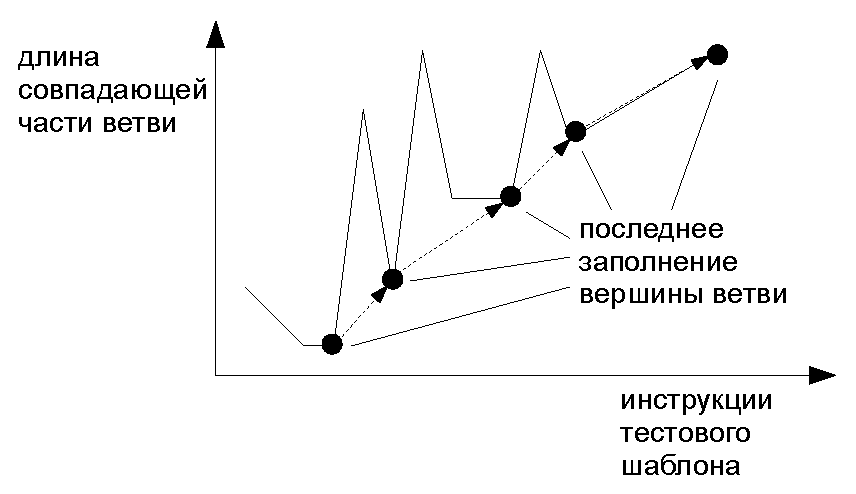
\includegraphics[width=0.6\textwidth]{2.theor/plru-useful}\\
  \caption{Заполнение ветви черными вершинами в стратегии вытеснения
  \PseudoLRU}\label{plru-useful}
\end{figure}

Рассмотрим в качестве метрики вытеснения для стратегии вытеснения
\PseudoLRU длину черной части ветви, начиная от листовых вершин к
корню дерева. Причем вершина будет учитываться в метрике как черная
не в тот момент, когда ее перекрашивают, а в тот момент, когда это
ее последнее покрашивание в черный цвет. Если таким образом будет
закрашена вся ветвь целиком перед кэш-промахом, то листовая вершина
будет вытеснена. Представленный на рисунке~\ref{plru-useful} шаблон
успевает
покрасить 5 вершин ветви в черный цвет. %Полезные инструкции
%объединены в ломаную, которую далее будем называть \emph{лестницей},
%а ее элемент \emph{ступенью лестницы}.

\begin{utv}
Инструкция считается полезной в случае стратегии вытеснения
\PseudoLRU, если все последующие обращения затрагивают только те
вершины ветви, которые расположены выше вершины, перекрашиваемой в
данный момент в черный цвет.
\end{utv}

Количество полезных инструкций, необходимых для вытеснения, зависит
от состояния ветви перед первой инструкций. Если обращение к тегсету
было в тестовом шаблоне, то для вытеснения нужно не менее $W$
полезных инструкций (длина ветви). Если обращения в тестовом шаблоне
не было (т.е. тегсет был в кэширующем буфере изначально), то для его
вытеснения может потребоваться менее $W$ полезных инструкций,
поскольку часть вершин покрашены в черный цвет изначально. Напомним,
что $W$ обозначает $\log_2 w$.

Отличие этой метрики вытеснения от метрики вытеснения для \LRU
является \emph{немонотонность}. Это означает, что полезные
инструкции надо считать для каждого кэш-промаха заново ---
инструкции между двумя соседними кэш-промахами могут забелить
несколько вершин ветви, что уменьшит метрику вытеснения
(см.рис.~\ref{nonmonotonic}). Метрика для \LRU является монотонной,
потому что инструкции между кэш-промахами не могут уменьшить метрику
вытеснения -- либо не меняют, либо увеличивают ее, сдвигая
вытесняемый тегсет к концу списка \LRU (см. рис.~\ref{monotonic}).
Таким образом, ограничение, описывающее стратегию вытеснения
\PseudoLRU, будет представлено дизъюнкцией ограничений по всем
предыдущим кэш-промахам.

\begin{figure}[h] \center
  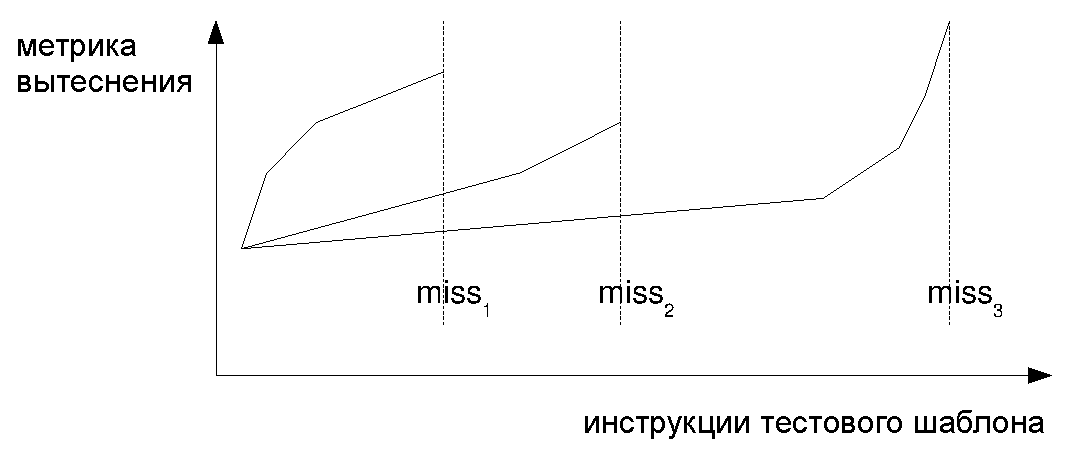
\includegraphics[width=0.6\textwidth]{2.theor/nonmonotonic}\\
  \caption{Немонотонная метрика вытеснения}\label{nonmonotonic}
\end{figure}

\begin{figure}[h] \center
  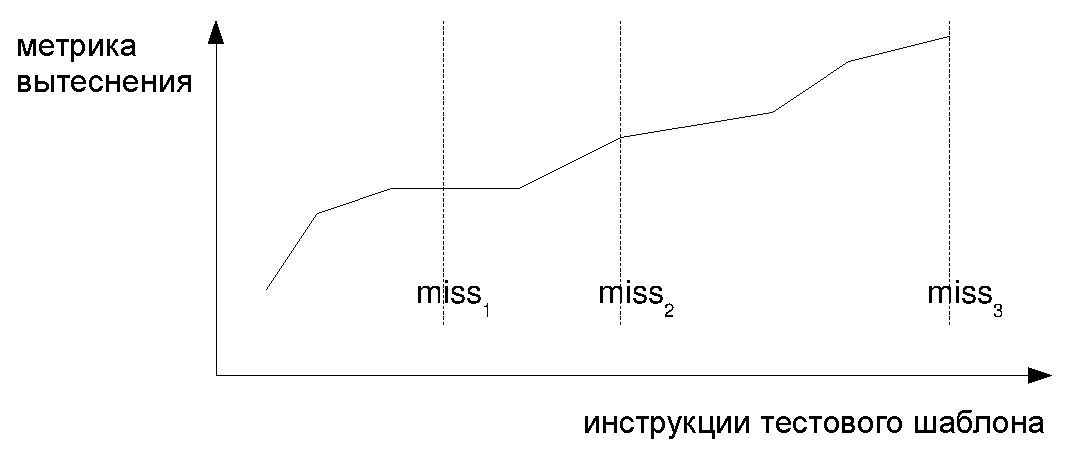
\includegraphics[width=0.6\textwidth]{2.theor/monotonic}\\
  \caption{Монотонная метрика вытеснения}\label{monotonic}
\end{figure}

Осталось записать понятие полезной инструкции для \PseudoLRU в виде
ограничений. Напомню, что каждый тегсет кроме своего значения $x_i$
снабжен позицией $\pi_i$ ($\pi_i \in \{0..w{-}1\})$. Пусть считается
функция полезности тегсета $(x_i, \pi_i)$ относительно тегсета
$(x,\pi)$. Пусть выбрана некоторая инструкция с кэш-промахом между
$i$'й и вытесняющей. Пусть $(x_{i+1},\pi_{i+1})$,
$(x_{i+2},\pi_{i+2}), ~\dots,$ $(x_m, \pi_m)$ -- тегсеты с позициями
инструкций, расположенными между $(x_i, \pi_i)$ и выбранным
кэш-промахом, а $(x_{i+1},\pi_{i+1}), ..., (x_n, \pi_n)$ -- тегсеты
с позициями инструкций, расположенными между $(x_i, \pi_i)$ и $(x,
\pi)$. Тогда $(x_i, \pi_i)$ будет полезным, если выполнены
одновременно три условия:
\begin{itemize}
\item $x \notin \{x_i, x_{i+1}, ..., x_n\}$ -- инструкция
расположена после последнего обращения к вытесняемому тегсету;
\item $R(x) = R(x_i)$ -- инструкция принадлежит тому же региону;
\item $P(\pi_i \oplus \pi,~\pi_{i+1} \oplus \pi) \wedge ... \wedge
P(\pi_i \oplus \pi,~\pi_{m-1} \oplus \pi)$ -- все последующие
обращения должны пересекаться только в более верхних частях ветви
(это выражает предикат $P$ для пары векторов); предикат $P(\delta_i,
\delta_j)$ истинен тогда и только тогда, когда количество старших
нулевых бит у $\delta_i$ больше количества старших нулевых бит у
$\delta_j$, иными словами, только и только тогда, когда существует
$k$ такое, что $\delta_i < 2^k \leqslant \delta_j$; с использованием
битовых операций этот предикат можно записать в следующем виде:
$P(\delta_i, \delta_j) \equiv (\delta_j
> \delta_i~~\wedge~~\delta_j \oplus \delta_i > \delta_i)$, сравнения
беззнаковые.
\end{itemize}

Таблица~\ref{plru_table} содержит ограничения для разных случаев
кэш-попаданий и кэш-промахов (см. утверждение~\ref{hit_miss_human}).
В каждое из них включается ограничение на количество полезных
инструкций согласно предлагаемой методике использования функций
полезности. Полезности считаются относительно некоторого кэш-промаха
(для их перебора используется сокращение $x_m : \mbox{miss}$). Теорема,
доказывающая корректность приведенных в таблице~\ref{plru_table}, приведена
и доказана в приложении~\ref{proofs}.


\subsection{Разрешение уравнений, описывающих стратегии вытеснения}

Ограничения, которые предлагается генерировать для описания тестовых
ситуаций в кэширующих буферах, можно разделить на две группы:
ограничения на конечные множества тегсетов и \emph{ограничения
мощности}.

Ограничения вида $C_1 \leqslant \sum_{i=1}^n a_i \leqslant C_2$, где
$C_1, C_2$ -- неотрицательные целые числа, а $a_i$ принимают
значения 0 или 1, называются \emph{ограничениями мощности}
(cardinality constraints)~\cite{smt_debugging, PiskacK08, KuncakR07,
Revesz05}. Речь идет об ограничении размера некоторого множества
элементов, возможно, заданного с помощью характеристической функции.
В~\cite{smt_debugging} проведено исследование способов записи
ограничений мощности и показано, что от формы записи зависит
эффективность разрешения этих ограничений. Например, ограничения
мощности можно рассматривать, как компактную форму записи уравнения
вида $\bigvee_{C_1 \leqslant C \leqslant C_2} \sum_{i=1}^n a_i = C$,
где равенство есть
\begin{itemize}
\item тождественная ложь, если $C < 0$ или $C > n$;
\item конъюнкция $\bigwedge_{1\leqslant i\leqslant n} (a_i = 0)$,
если $C = 0$;
\item дизъюнкция по всевозможным выборкам индексов $i_1, ..., i_C$, где
для каждого индекса $i_k$ справедливы свойства $1 \leqslant i_k
\leqslant n$ и $i_k < i_{k+1}$, конъюнкций $\bigwedge_{i_k} (a_{i_k}
= 1)$, если $1 \leqslant C \leqslant n$.
\end{itemize}

Задача организации особой процедуры разрешения ограничений не
входила в проводимое исследование, поэтому были использованы
имеющиеся инструменты решения систем уравнений и неравенств.

После устранения ограничений мощности в формуле остаются только
ограничения на конечные множества тегсетов: принадлежности и
непринадлежности тега конечному множеству тегсетов и равенства и
неравенства битовых полей тегсетов. Поскольку конечные множества
тегсетов известны (заданы перечислением тегсетов, которые в входят в
это множество), то ограничения принадлежности и непринадлежности
могут быть переписаны без использования этих отношений. Отношение
принадлежности $x \in \{x_1, x_2, ..., x_n\}$ может быть переписано
в виде дизъюнкции $(x = x_1) \vee (x = x_2) \vee ... \vee (x =
x_n)$, а отношение непринадлежности $x \notin \{x_1, x_2, ...,
x_n\}$ -- в виде конъюнкции $(x \neq x_1) \wedge (x \neq x_2) \wedge
... \wedge (x \neq x_n)$.

В результате получается предикат, в котором переменными величинами
являются неотрицательные целые числа с конечной областью значений
(тегсеты), над переменными возможны операции получения битового
поля, в предикате используется отношение равенства и неравенства над
битовыми полями. Кроме того, этот предикат задается с использованием
ограничений мощности.

Для разрешения такого рода предикатов можно было бы разрабатывать
собственные процедуры распространения ограничений, но это свело бы
на нет все усилия по выработке собственного представления стратегии
вытеснения. Однако предлагаемые ограничения могут быть тривиальным
образом выражены на языке теорий, для которых существуют эффективные
разрешающие процедуры (битовые строки, неинтерпретируемые функции).
Поэтому для записи и разрешения этих ограничений могут быть
использованы SMT-инструменты~\cite{Z3}.

%%%%%%%%%%%%%%%%%%%%%%%%%%%%%%%%%%%%%%%%%%%%%%%%%%%%%%%%%%%%%%%%%%

\pagebreak
\section{Ограничения, описывающие тестовые ситуации в некоторых
частных случаях, для стратегии вытеснения \LRU}

\subsection{Тестовые шаблоны без кэш-промахов}

В случае тестовых шаблонов, в которых нет кэш-промахов, нет ни
вытесняющих, ни вытесняемых тегсетов. Поэтому в таких шаблонов
уравнения для кэш-попаданий имеют очень простой вид:

$$
\left\{
\begin{array}{l}
x \in D\\
... (\mbox{тестовые ситуации на остальные буферы})\\
\end{array}
\right.
$$

\subsection{Тестовые шаблоны без кэш-попаданий}

В случае тестовых шаблонов, в которых нет кэш-попаданий, надо
генерировать ограничения для вытесняющих и лишь иногда для
вытесняемых тегсетов. А именно, вытесняемый тегсет требуется лишь в
том случае, когда кэш-промах вносит в кэширующий буфер ранее
вытесненный тегсет. В этом случае для вытесняемого тегсета известен
домен, что позволяет построить уравнения обозримого размера. Кроме
того, поскольку отсутствуют кэш-попадания, повторные обращения к
вытесняемым тегсетам (кроме кэш-промаха, который их может внести в
кэширующий буфер) невозможны, что также упрощает генерируемые
уравнения.

В результате получается, что вытесняющий тегсет описывается в
тестовом шаблоне без кэш-попаданий следующей системой уравнений:
$$
F'(x) \vee F''(x) \vee \bigvee_{\lambda_\delta \in D} F'''(x, \lambda_\delta)
$$

где

$$F'(x) \equiv (x \notin D \wedge x \notin \{x_1, ..., x_n\})$$

$$F''(x) \equiv (x \in \{x_1, ..., x_n\} \wedge \sum_{i=1}^n u''(x_i) \geqslant w)$$

$$u''(x_i) \equiv (x\notin \{x_i, ..., x_n\} \wedge R(x_i) = R(x))$$

$$F'''(x, \lambda_\delta) \equiv (x = \lambda_\delta \wedge x \notin
\{x_1, ..., x_n\} \wedge \sum_{i=1}^n (R(x_i) = R(x)) \geqslant w -
\delta + 1)$$

\subsection{Короткие тестовые шаблоны}

Будем называть тестовый шаблон \emph{коротким}, если в нем не более
$w$ инструкций обращения к памяти. Очевидно, что любой короткий
тестовый шаблон является простым. Из 7 случаев для коротких тестовых
шаблонов остается всего 5 (первые два можно еще объединить в более
компактную систему уравнений). В таблице~\ref{short_templates_table}
предъявлены функции полезности и ограничения для коротких тестовых
шаблонов в случае стратегии вытеснения \LRU. Соответствующая теорема
корректности этих ограничений сформулирована и доказана в приложении~\ref{proofs}.

\begin{table}[t]
\begin{tabular}{|c|c|c|c|}
\hline  & \centering случай &
\begin{tabular}{c}переменная\\перебора\end{tabular} & система \\
\hline \hline \multirow{-2}{*}{\rotatebox{90}{кэш-попадание}} &
\makecell[c{p{0.3\textwidth}}]{тегсет находится в начальном
состоянии буфера и он всё ещё не вытеснен} & $\lambda_\delta \in D$
&
$\left\{\begin{array}{l} x = \lambda_\delta\\
\sum\limits^n_{i=1} u(x_i) \leqslant w - \delta
\end{array}\right.$ \\ \hhline{~|---}
& \makecell[c{p{0.3\textwidth}}]{тегсет уже встречался в шаблоне} &
-- & $x \in \{x_1, ..., x_n\}$
\\ \hline \hline \multirow{6}{*}{\rotatebox{90}{кэш-промах}}
& \makecell[c{p{0.3\textwidth}}]{тегсет встречается впервые} & -- &
$\left\{\begin{array}{l} x \notin D\\
x \notin \{x_1, ..., x_n\}\\
\end{array}\right.$\\ \hhline{~|---} &
\makecell[c{p{0.3\textwidth}}]{тегсет находился в начальном
состоянии буфера и был вытеснен} & $\begin{array}{c}\lambda_\delta
\in D,\\\delta \geqslant w-n+1\end{array}$ &
$\left\{\begin{array}{l} x = \lambda_\delta\\
x \notin \{x_1, ..., x_n\}\\
\sum\limits^n_{i=1} u(x_i) > w - \delta\\
\end{array}\right.
$ \\ \hline
\end{tabular}

%где функция полезности определена следующим образом:
$$u(x_i) \equiv
\left\{\begin{array}{l} x_i \in \{ \lambda_{\delta+1}, ...,
\lambda_w\}~\wedge~x_i \notin \{x_1, ..., x_{i-1}\}, \mbox{если}~S_i
= \mbox{hit}\\
R(x_i) = R(x), \mbox{если}~S_i = \mbox{miss}
\end{array}\right.
$$
\caption{Таблица систем уравнений для тестовых ситуаций в кэширующих
буферах для коротких тестовых шаблонов в случае стратегии вытеснения
\LRU}\label{short_templates_table}
\end{table}



%\begin{landscape}
%\begin{table}
%\begin{tabular}{|c|c|c|c|c|c|}
%\hline  & \centering случай &
%\begin{tabular}{c}переменная\\перебора\end{tabular} & система &
%\begin{tabular}{c}функция\\полезности\\для кэш-\\попадания\end{tabular} &
%\begin{tabular}{c}функция\\полезности\\для кэш-\\промаха\end{tabular} \\
%\hline \hline \multirow{-2}{*}{\rotatebox{90}{кэш-попадание}} &
%\makecell[c{p{0.3\textwidth}}]{тегсет находится в начальном
%состоянии буфера и он всё ещё не вытеснен} & $\lambda_\delta \in
%D$ &
%$\left\{\begin{array}{l} x = \lambda_\delta\\
%\sum\limits^n_{i=1} u(x_i) \leqslant w - \delta
%\end{array}\right.
%$ &
%\begin{tabular}{c}
%$x_i \in \{ \lambda_{\delta+1}, ..., \lambda_w\}$\\
%$\wedge~x_i \notin \{x_1, ..., x_{i-1}\}$
%\end{tabular}
%& $R(x_i) = R(x)$
%\\ \hhline{~|-----}
%& \makecell[c{p{0.3\textwidth}}]{тегсет уже встречался в шаблоне} &
%-- & $x \in \{x_1, ..., x_n\}$ & -- & --
%\\ \hline \hline \multirow{6}{*}{\rotatebox{90}{кэш-промах}}
%& \makecell[c{p{0.3\textwidth}}]{тегсет встречается впервые} & -- &
%$\left\{\begin{array}{l} x \notin D\\
%x \notin \{x_1, ..., x_n\}\\
%\end{array}\right.
%$ & -- & -- \\ \hhline{~|-----} &
%\makecell[c{p{0.3\textwidth}}]{тегсет находился в начальном
%состоянии буфера и был вытеснен} &
%$\begin{array}{c}\lambda_\delta \in D,\\\delta \geqslant
%w-n+1\end{array}$ &
%$\left\{\begin{array}{l} x = \lambda_\delta\\
%x \notin \{x_1, ..., x_n\}\\
%\sum\limits^n_{i=1} u(x_i) > w - \delta\\
%\end{array}\right.
%$ &
%\begin{tabular}{c}
%$x_i \in\{\lambda_{\delta+1}, ..., \lambda_w\}$\\
%$\wedge~x \notin \{x_1, ..., x_{i-1}\}$\\
%\end{tabular}
%&
%\begin{tabular}{c}
%$R(x_i) = R(x)$\\
%\end{tabular}
%\\ \hline
%\end{tabular}
%\caption{Таблица систем уравнений для тестовых ситуаций в кэширующем буфере
%для коротких тестовых шаблонов в случае стратегии вытеснения
%\LRU}\label{short_templates_table}
%\end{table}
%\end{landscape}


\subsection{Генерация тестовых данных для кэш-памяти, содержащей
<<грязные>> ячейки}

Любая ячейка в кэш-памяти может быть помечена \emph{грязной}
(\emph{invalid}). Это означает, что данные, находящиеся в кэширующем
буфере по этому адресу, не могут использоваться в качестве данных,
хранящихся в памяти по этому адресу.

Рассмотренные ранее в этой работе случаи не учитывали грязные ячейки
кэширующем буфере, хотя они зачастую присутствуют в микропроцессоре
после его запуска -- с таким состоянием кэширующего буфера работают
первые после запуска микропроцессора инструкции.

Кэш-попадание возникает в том случае, когда требуемые данные
присутствуют среди <<чистых>> ячеек кэширующего буфера. Кэш-промах
возникает в том случае, когда требуемых данных нет среди <<чистых>>
ячеек. Причем при наличии <<грязных>> ячеек вытеснения может и не
произойти. А именно, если все ячейки набора, с которым работает
инструкция, являются <<чистыми>>, то происходит вытеснение согласно
стратегии вытеснения, остальные наборы не меняются. Если же среди
ячеек набор есть <<грязные>> ячейки, то вытеснение не происходит, а
на место одной из <<грязных>> ячеек помещаются данные из основной
памяти по заданному адресу и ячейка объявляется <<чистой>>.
Остальные ячейки не меняются. В стратегии вытеснения \LRU эта бывшая
<<грязная>> ячейка становится самой новой.

Для генерации тестовых данных для кэширующих буферов с грязными
ячейками предлагается применять ограничения с функциями полезности.
Примечательно, что наличие грязных ячеек не меняет качественно
систему уравнений.

В данном разделе рассматривается случай, когда начальное состояние
микропроцессора известно. Кроме того, рассматриваемый случай
учитывает отсутствие инструкций в тестовом шаблоне, которые
превращали бы <<чистые>> ячейки в <<грязные>> (т.е. все такие
изменения должны делаться явно вне тестовых шаблонов).

\subsubsection{случай полностью-ассоциативного кэширующего буфера}

В случае полностью-ассоциативных кэширующих буферов очевидно, что
первые кэш-промахи будут заполнять <<грязные>> ячейки. Пусть $N$ --
количество <<грязных>> ячеек в начальном состоянии кэширующего
буфера, а $L_0$ -- начальное состояние (выражение) кэширующего
буфера (только <<чистые>> ячейки). Тогда для тестовых ситуаций надо
генерировать такие ограничения ($L$ -- выражение для состояния
кэширующего буфера перед исполнением инструкции, $L'$ -- выражение
для состояния кэширующего буфера после исполнения инструкции):
\begin{itemize}
\item для \emph{кэш-попадания} hit($x$) генерируются ограничения
$$
\left\{
\begin{array}{l}
x \in L\\
L' \equiv L\\
\end{array}
\right.
$$

\item для \emph{кэш-промаха} miss($x$), если это один из первых $N$
кэш-промахов, генерируются ограничения:
$$
\left\{
\begin{array}{l}
x \notin L\\
L' \equiv L \cup \{x\}\\
\end{array}
\right.
$$

\item для \emph{кэш-промаха} miss($x$), являющегося по счету более
чем $N$'м кэш-промахом тестового шаблона, генерируются ограничения:
$$
\left\{
\begin{array}{l}
x \notin L\\
x' \in L\\
L' \equiv L\setminus\{x'\} \cup \{x\}\\
displaced(x', L)\\
\end{array}
\right.
$$
\end{itemize}

Предикат $displaced(x', L)$ истинен, если $x'$ является вытесняемым
тегом в текущем состоянии кэширующего буфера $L$. Для стратегии
вытеснения \LRU этот предикат может быть записан с использованием
тех же диапазонов вытеснения, что и для кэширующего буфера без
<<грязных>> ячеек (см.п.~\ref{LRU_constraints}). А именно, диапазон
вытеснения начинается на инструкции, которая последний раз перед
вытеснением тега обращается к нему. Тогда между этой инструкцией и
инструкцией, вытесняющей $x$, должны быть обращения ко всем
остальным тегам текущего состояния кэширующего буфера. Эта логика
может быть записана в виде тех же уравнений, что и в
пункте~\ref{LRU_constraints}. Нетрудно проверить, что для
кэширующего буфера с <<грязными>> ячейками остается справедливой
лемма о невложенных диапазонах вытеснения, что доказывает
корректность использования ограничений из
пункта~\ref{LRU_constraints} для кэширующего буфера с <<грязными>>
ячейками.

\subsubsection{случай наборно-ассоциативного кэширующего буфера}

В этом пункте будет показано, что ограничения для кэширующего
буфера, начальное состояние которого содержит <<грязные>> ячейки,
качественно не отличаются от ограничений для кэширующего буфера без
<<грязных>> ячеек.

Аналогично тому, как это делалось для кэширующих буферов без
<<грязных>> ячеек, для тестовых ситуаций на кэширующие буферы с
<<грязными>> ячейками тоже возможно следующее исчерпывающее
выделение случаев:
\begin{itemize}
\item кэш-попадание тега:
    \begin{enumerate}
    \item данный тег находился в начальном состоянии кэширующего буфера и не был
    вытеснен к моменту данной инструкции;
    \item данный тег был внесен в кэширующий буфер одной из инструкций
    кэш-промаха и с тех пор не был вытеснен;
    \end{enumerate}
\item кэш-промах тега:
    \begin{enumerate}
    \item данный тег не встречался ранее (не находился в начальном
    состоянии кэширующего буфера и не был внесен какими-либо кэш-промахами);
    \item данный тег был ранее вытеснен из кэширующего буфера и с тех пор
    не был внесен в кэширующий буфер вновь.
    \end{enumerate}
\end{itemize}

Соответствующие ограничения приведены в
таблице~\ref{dirty_hit_miss_table}.


В таблице~\ref{dirty_hit_miss_table} символ $\Delta$ означает
количество <<чистых>> ячеек в начальном состоянии того региона, про
который идет речь в уравнении. На самом деле $\Delta$ есть функция
региона ($\Delta = \Delta(\lambda_\delta)$), но для сокращения
записи оставлен только функциональный символ. Кроме того, в
приведенных уравнениях домен переменной включает только <<чистые>>
ячейки.

Сходства уравнений (со случаем кэширующих буферов без <<грязных>>
ячеек) удалось добиться за счет рассмотрения <<грязных>> ячеек, как
ячеек с наименьшим счетчиком \LRU, которые не участвуют в
определении нахождения тега в кэширующих буферах. Поэтому в функциях
полезности участвуют множества не $\{\lambda_{\delta+1}, ...,
\lambda_w\}$, а множества $\{\lambda_{\delta+1}, ...,
\lambda_\Delta\}$. Все <<чистые>> ячейки получили первые индексы,
т.е. индексы всех от 1 до $\Delta$.

%\begin{theorem}[корректность использования функций полезности для
%записи \LRU в случае наличия <<грязных>> ячеек в начальном состоянии
%кэширующего буфера] Тестовая программа, построенная по ограничениям,
%которые сгенерированы с использованием предъявленных в
%таблице~\ref{dirty_hit_miss_table} функций полезности, в случае
%наличия <<грязных>> ячеек в начальном состоянии кэширующего буфера
%удовлетворяет своему тестовому шаблону.
%\end{theorem}
%\begin{proof}
%  //TODO
%\end{proof}

Для приведенных ограничений также могут быть применены эвристики,
сокращающие их количество, которые были упомянуты для кэширующих
буферов без <<грязных>> ячеек. Кроме того, в данном случае возможна
дополнительная эвристика \emph{ограничение на $\delta$}: если
$\delta + 1 < \Delta$, то функция полезности, в которую входит
множество $\{\lambda_{\delta+1}, ..., \lambda_\Delta\}$, равна 0.

\subsection{Функции полезности для зеркальной генерации тестовых
данных}

Рассмотрим ограничения, генерируемые для тестовых шаблонов
зеркальным методом с использованием функций полезности. По сравнению
с представленными ограничениями (см. табл.~\ref{hit_miss_table})
зеркальная генерация имеет свои особенности:
\begin{enumerate}
  \item множества констант (как, например, $L, D$) не используются,
  поэтому в ограничениях будут отсутствовать соответствующие им
  случаи;
  \item так как теги инструкций тестового шаблона должны появиться
  среди инициализирующей последовательности, то для вытеснения
  требуется $w-1$ инструкций, где $w$ -- ассоциативность кэширующего буфера;
  \item учет полезных инструкций начинается уже в инициализирующей
  последовательности, тем самым необходимо сформулировать функцию
  полезности для инициализирующих инструкций.
\end{enumerate}

Следующая теорема описывает функцию полезности для инициализирующих
инструкций и описывает ограничения, генерируемые для тестовых
шаблонов зеркальным методом с использованием функций полезности
(количество инициализирующих инструкций зафиксировано, оно будет
обозначено параметром $m$):

\begin{theorem}[Корректность ограничений, генерируемые зеркальным методом с
использованием функций полезности для
\LRU]\label{correct_mirror_LRU} Пусть $t_1, t_2, ..., t_m$ -- теги
инициализирующей последовательности, $x$ -- текущий тег тестового
шаблона, $x_1, x_2, ..., x_n$ -- теги предыдущих инструкций
тестового шаблона, причем $x \in \{t_1, ..., t_m, x_1, ..., x_n\}$ и
$\{t_1, ..., t_m\}$ --- все разные. Тогда $x$ не вытеснен согласно
определению на списках тогда и только тогда, когда
$$\sum\limits_{i=1}^{m+n} u_x(s_i) < w$$
где последовательность $s \equiv \langle t_1, ..., t_m, x_1, ...,
x_n\rangle$, а функция полезности определена следующим образом:
$$u_x(s_i) \equiv (x \notin \{s_i, ..., s_{m+n}\} \wedge
R(x) = R(s_i) \wedge s_i \notin\{s_{i+1},..., s_{m+n}\})$$

%$$\sum\limits_{i=1}^m \tilde{u}_x(t_i) + \sum\limits_{i=1}^n u_x(x_i) < w$$
%где функции полезности определены следующим образом:
%$$\begin{array}{c}
%\tilde{u}_x(t_i) \equiv (x \notin \{t_i, ..., t_m, x_1, ..., x_n\}
%\wedge R(x) = R(t_i))\\u_x(x_i) \equiv (x \notin \{x_i, ..., x_n\}
%\wedge R(x) = R(x_i))\end{array}$$

%$$\begin{array}{c}u_x(x_i) \equiv (x \notin \{x_i, ..., x_n\} \wedge R(x) =
%R(x_i)), \mbox{если}~S_i=\mbox{miss}\end{array}$$
%$$\begin{array}{c}u_x(x_i) \equiv (x \notin \{x_i, ..., x_n\} \wedge R(x) =
%R(x_i) \wedge \sum\limits_{j=1}^{m} \tilde{c}_{x_i}(t_j) = 0
%\wedge \sum\limits_{j=1}^{i-1} c_i(x_j) = 0),\\
%\mbox{если}~S_i=\mbox{hit}\end{array}$$
%$$c_i(x_j) \equiv (x \notin \{x_j, ..., x_{i-1}\} \wedge x_i = x_j)$$
%$$\tilde{c}_{x_i}(t_j) \equiv (x \notin \{t_j, ..., t_m, x_1, ..., x_{i-1}\} \wedge x_i = t_j)$$
\end{theorem}
\begin{proof}
//TODO написать правильное доказательство

сумма полезных - это количество различных тегов, тогда полезными будем считать инструкции тестового шаблона, которые обращаются к разным тегам, при этом ко всем различным тегам есть инструкция; различные - например, последние; отсюда и функция полезности.

%Воспользуемся леммой~\ref{hit_II}. При этом в качестве
%последовательности тегов тестового шаблона в этой лемме рассмотрим
%последовательность $t_1, t_2,~\dots,~t_m,~x_1,~x_2,~\dots,~x_n$.
%Согласно лемме тестовая ситуация на $x$ выполнена при
%соответствующем условии на сумму функций полезности от элементов
%этой последовательности. Функции полезности для
%$x_1,~x_2,~\dots,~x_n$ без изменений переходят из формулировки
%леммы~\ref{hit_II} в данную теорему. Функцию полезности для $t_1,
%t_2,~\dots,~t_m$ из формулировки леммы~\ref{hit_II} получить нельзя,
%поскольку неизвестна тестовая ситуация на эти теги. Однако, вспомнив
%определение полезной инструкции, функцию полезности для этих тегов
%получить несложно. А именно, тег $t_i$ будет полезным, если он
%продвигает $x$ к концу списка \LRU после последнего обращения к $x$.
%Если после последнего обращения к $x$ сам тег $t_i$ встречается
%впервые, то он будет полезным (см. доказательство
%леммы~\ref{hit_II}). Если же после последнего обращения к $x$ $t_i$
%встречается не в первый раз, то он не двигает $x$ к концу списка,
%что, тем самым, означает бесполезность $t_i$. Но поскольку все $t_i$
%разные, то повторное обращение возможно лишь среди
%$x_1,~x_2,~\dots,~x_n$ -- поэтому в функцию полезности для этих
%тегов добавлено отличие от $t_1,~t_2,~\dots,~t_m$.
\end{proof}
%\begin{sld}[Корректность ограничений, генерируемые зеркальным методом с
%использованием функций полезности для полностью ассоциативного \LRU
%буфера] Пусть $t_1, t_2, ..., t_m$ -- теги инициализирующей
%последовательности, $x$ -- текущий тег тестового шаблона, $x_1, x_2,
%..., x_n$ -- теги предыдущих инструкций тестового шаблона, причем $x
%\in \{t_1, ..., t_m, x_1, ..., x_n\}$ и $\{t_1, ..., t_m\}$ --- все
%разные. Тогда $x$ не вытеснен из полностью ассоциативного буфера
%согласно определению на списках тогда и только тогда, когда
%$$x \in \{s_{m+n-w+1}, ..., s_{m+n}\}$$ где последовательность $s
%\equiv \langle t_1, ..., t_m, x_1, ..., x_n\rangle$.
%\end{sld}
%\begin{proof}
%  //TODO
%\end{proof}

Из теоремы~\ref{correct_mirror_LRU} следует система уравнений для
описания тестовой ситуации $S$ тега $x$, генерируемая зеркальным
методом с использованием функций полезности для \LRU (функции
полезности приведены в формулировке
теоремы~\ref{correct_mirror_LRU}):
\begin{itemize}
\item если $S$ = hit, то
$$
\left\{\begin{array}{l} x \in \{t_1, ..., t_m, x_1, ..., x_n\}\\
\sum\limits_{i=1}^m u_x(t_i) + \sum\limits_{i=1}^n u_x(x_i) < w\\
\{t_1, ..., t_m\} - \mbox{все разные}\\
\end{array} \right.
$$
\item если $S$ = miss, то
$$
\left\{\begin{array}{l} x \in \{t_1, ..., t_m, x_1, ..., x_n\}\\
\sum\limits_{i=1}^m u_x(t_i) + \sum\limits_{i=1}^n u_x(x_i)
\geqslant w\\
\{t_1, ..., t_m\} - \mbox{все разные}\\
\end{array} \right.
$$
\end{itemize}

%Стоит заметить, что функции полезности добавили новое дополнительное
%условие на теги инициализирующих инструкций: они должны быть
%различными. В этом выражается свойство <<простоты>> инициализирующей
%последовательности, эта последовательность не должна содержать
%сложной внутренней последовательности изменений состояния
%кэширующего буфера.

\subsection{Зеркальный метод генерации ограничений для кэш-памяти
первого и второго уровня}

Рассмотрим один часто встречающийся случай кэширующих буферов,
инициализация которого может вызывать трудности. Речь идет о
кэш-памяти второго уровня. Зачастую кэш-память второго уровня не
может быть инициализирована отдельно от остальных подсистем
микропроцессора, обычно оно связано с изменением кэш-памяти первого
уровня. Это создает дополнительные сложности при формулировании
ограничений методом зеркальной генерации, поскольку инициализирующая
последовательность должна подготавливать сразу два кэширующих буфера
одновременно -- кэш-память первого уровня и кэш-память второго
уровня. Кроме того, зачастую кэш-память второго уровня является
совместной для хранения в ней данных и инструкций. Поэтому на
инициализацию кэш-памяти второго уровня влияют и сами
инициализирующие инструкции, и даже адрес расположения тестовой
программы в памяти (от него зависит виртуальный адрес инструкций, а
значит теги и индексы при обращении к кэш-памяти инструкций).

Если принять дополнительное требование (и оно даст решение), что в
кэш-памяти второго уровня наборы, используемые для доступа к
инструкциям, не пересекаются с наборами, используемыми для доступа к
данным, то генерируемые ограничения упрощаются (кэширование
инструкций можно вообще не учитывать). С точки зрения зеркальной
генерации это означает, что надо сформулировать требования на
инициализирующую последовательность. Напомню, что одним из ключевых
требований является произвольность начального состояния
(содержимого) кэш-памяти.

Предположим, что обращение к кэш-памяти второго уровня
осуществляется при кэш-промахе в кэш-памяти первого уровня и
кэш-память не является virtually indexed virtually
tagged~\cite{HennessyPatterson3rd}. Для составления ограничений с
использованием функций полезности необходимо знать, которые
инструкции среди инициализирующей последовательности действительно
обращаются в кэш-память второго уровня (иными словами, в каких
инструкциях среди инициализирующей последовательности происходит
кэш-промах при обращении к кэш-памяти первого уровня). Возможным
решением было бы перебирать всевозможные распределения тестовых
ситуаций в кэш-памяти первого уровня на элементах инициализирующей
последовательности (с предварительной подготовкой этих тестовых
ситуаций). Однако следующая лемма~\ref{special_initialization_L2}
показывает, что для любого такого произвольного распределения
тестовых ситуаций в кэш-памяти первого уровня существует решение со
специальным распределением тестовых ситуаций. Это позволяет
перебирать только такие специальные распределения тестовых ситуаций
в кэш-памяти первого уровня. При этом вычислительная сложность
процедуры поиска инициализирующей последовательности, дающей
решение, изменяется от экспоненциальной от длины тестового шаблона к
полиномиальной, что показывает лемма~\ref{max_k_h} (ее доказательство
приведено в приложении~\ref{proofs}):
\begin{lemma}[Верхняя оценка длины специальной инициализирующей
последовательности для стратегии вытеснения \LRU]\label{max_k_h} \MaxUpperBoundLRU
\end{lemma}
\begin{sld}
$$m = O(n)$$ где $m$ --- длина специальной инициализирующей
последовательности, $n$ -- количество инструкций тестового шаблона.
\end{sld}

Для получения инициализирующей программы минимальной длины, можно
применять сначала двоичный поиск суммы $k+h$ с применением
дальнейшего поиска допустимых значений $k$ и $h$.

%%%%%%%%%%%%%%%%%%%%%%%%%%%%%%%%%%%%%%%%%%%%%%%%%%%%%%%%%%%%%%%%%%%%%
